\documentclass[a4paper,12pt]{report}

\nocite{*}

\newcommand{\nameInitial}{
    \textcolor{black}{G. Allen}
}
\newcommand{\nameFull}{
    \textcolor{black}{Gary Allen}
}
\newcommand{\stNumber}{
    \textcolor{black}{23905093}
}
\newcommand{\myDate}{\textcolor{black}{\today}
}
\newcommand{\signature}{frontmatter/figures/Signature}

% Page layout
\usepackage[left=2.2cm,right=2.2cm,top=2.2cm,bottom=2.2cm]{geometry}

% Figures
\usepackage[margin=\the\parindent,small,bf,sf]{caption}
\usepackage{graphicx}
\usepackage{pdfpages}
\setlength{\abovecaptionskip}{7.5pt}  % spacing above and below captions
\newcommand*{\WaterMark}[2][0.2\paperwidth]{\AddToShipoutPicture*{\AtTextCenter{\parbox[c]{0pt}{\makebox[0pt][c]{\includegraphics[width=#1]{#2}}}}}}
\usepackage{subcaption}

% Items and Enums
\usepackage{enumitem}
\renewcommand{\labelitemii}{$\circ$}

% Font and text
\usepackage[afrikaans,english]{babel}
\usepackage{microtype}
\usepackage{setspace}
\usepackage{lmodern}
\newcommand{\myemph}[1]{{\sffamily\bfseries#1}}
\sloppy
\onehalfspacing
\usepackage{siunitx}
\usepackage{lipsum}
\usepackage[super]{nth}

% Headings
\usepackage[raggedright,sf,bf]{titlesec}
\titlelabel{\thetitle.\ }
\titleformat{\chapter}[display]{\huge\bfseries\sffamily}{\chaptertitlename\ \thechapter}{15pt}{\raggedright}
\titlespacing*{\chapter}{0pt}{0pt}{10pt}  % remove spacing before chapter headings

% Table of contents
\makeatletter
\let\originall@chapter\l@chapter
\def\l@chapter#1#2{\originall@chapter{{\sffamily #1}}{#2}}
\makeatother
\let \savenumberline \numberline
\def \numberline#1{\savenumberline{#1.}}

% Mathematics
\usepackage[cmex10]{amsmath}
\usepackage{amssymb}
\usepackage{cancel}
\DeclareMathOperator*{\argmax}{arg\,max}
\newcommand{\T}{^\textrm{T}}
\newcommand{\tr}{\textrm{tr}}
\renewcommand{\vec}[1]{\boldsymbol{\mathbf{#1}}}
\newcommand{\defeq}{\triangleq}

\makeatletter
\newcommand*{\inlineequation}[2][]{%
  \begingroup
    \refstepcounter{equation}%
    \ifx\\#1\\%
    \else
      \label{#1}%
    \fi
    \relpenalty=10000 %
    \binoppenalty=10000 %
    \ensuremath{%
      #2%
    }%
    ~\@eqnnum
  \endgroup
}
\makeatother

% Tables
\usepackage{booktabs}
\usepackage{tabularx}
\usepackage{multirow}
\newcommand{\mytable}{
    \centering
    \small
    \renewcommand{\arraystretch}{1.2}
    }
\renewcommand{\tabularxcolumn}[1]{m{#1}}
\newcolumntype{C}{>{\centering\arraybackslash}X}
\newcolumntype{L}{>{\raggedright\arraybackslash}X}

% Header and footer
\usepackage{fancyhdr}
\pagestyle{fancy}
\fancyhf{}
\renewcommand{\sectionmark}[1]{\markright{\normalsize \thesection.\ #1}}
\fancyhead[C]{\nouppercase{\textit{\rightmark}}}
\fancyhead[RO]{\thepage}

\fancyfoot{}
\setlength\headheight{14.5pt}
\renewcommand{\headrulewidth}{0pt}
\fancypagestyle{plain}{\fancyhead{}
                       \renewcommand{\headrulewidth}{0pt}
                       \fancyfoot[C]{\thepage}}

% Pseudo-code
\usepackage{algorithm}  % should go before \usepackage{hyperref}

% Table of contents and hyperlinks
\usepackage{hyperref}
\hypersetup{colorlinks=true,linktoc=all,citecolor=black,linkcolor=black}
\usepackage[nottoc]{tocbibind}

% Pseudo-code
\usepackage{algpseudocode}  % should go after \usepackage{hyperref}
\renewcommand{\thealgorithm}{\arabic{chapter}.\arabic{algorithm}} 
\captionsetup[algorithm]{labelfont={bf,sf},font=small,labelsep=colon}

% Bibliography
\usepackage{cite}  % automatically reorder inline citations
\bibliographystyle{IEEEtran}

% Fix titlesec issue
\usepackage{etoolbox}
\makeatletter
\patchcmd{\ttlh@hang}{\parindent\z@}{\parindent\z@\leavevmode}{}{}
\patchcmd{\ttlh@hang}{\noindent}{}{}{}
\makeatother
 \usepackage[normalem]{ulem}

\begin{document}

% Front matter
\graphicspath{{frontmatter/figures/}}
\pagenumbering{Alph}

\begin{titlepage}
\begin{center}


\includegraphics[width=8cm]{SU_logo_RGB_without_slogan.pdf}

\vfill

{\sffamily \bfseries \huge E344 Assignment 1 \par}

\vfill

{\large {\Large \nameFull} \\ \stNumber \par}

\vfill

\vfill

{Report submitted in partial fulfilment of the requirements of the module \\
Design (E) 344 for the degree Baccalaureus in Engineering in the Department of
Electrical and Electronic Engineering at Stellenbosch University. \par}

\vfill

%{\large {Supervisor}: Dr L. Skywalker} %\\
% Department of Electrical and Electronic Engineering \par}

\vfill

{\Large \myDate}
\end{center}
\end{titlepage}

\pagenumbering{roman}
\graphicspath{{frontmatter/figures/}}
\newpage
\pagestyle{plain}
\addcontentsline{toc}{chapter}{Declaration}
\makeatletter\@mkboth{}{Declaration}\makeatother

\centerline{
\includegraphics[width=8cm]{SU_horizontal_RGB.pdf}}
\vspace*{-10pt}

\section*{\centering Plagiaatverklaring / \textit{Plagiarism Declaration}}

\vspace*{5pt}

\begin{enumerate}
    \item Plagiaat is die oorneem en gebruik van die idees, materiaal en ander intellektuele eiendom van ander persone asof dit jou eie werk is.\\
    \textit{Plagiarism is the use of ideas, material and other intellectual property of another's work
        and to present is as my own.}
    
    \item Ek erken dat die pleeg van plagiaat 'n strafbare oortreding is aangesien dit 'n vorm van diefstal is.\\
    \textit{I agree that plagiarism is a punishable offence because it constitutes theft.}
    
    \item Ek verstaan ook dat direkte vertalings plagiaat is. \\
    \textit{I also understand that direct translations are plagiarism.}
    
    \item Dienooreenkomstig is alle aanhalings en bydraes vanuit enige bron (ingesluit die internet) volledig verwys (erken). Ek erken dat die woordelikse aanhaal van teks sonder aanhalingstekens (selfs al word die bron volledig erken) plagiaat is. \\
    \textit{Accordingly all quotations and contributions from any source whatsoever (including the internet) have been cited fully. I understand that the reproduction of text without quotation marks (even when the source is cited) is plagiarism}
    
    \item Ek verklaar dat die werk in hierdie skryfstuk vervat, behalwe waar anders aangedui, my eie oorspronklike werk is en dat ek dit nie vantevore in die geheel of gedeeltelik ingehandig het vir bepunting in hierdie module/werkstuk of 'n ander module/werkstuk~nie. \\
    \textit{I declare that the work contained in this assignment, except where otherwise stated, is my original work and that I have not previously (in its entirety or in part) submitted it for grading in this module/assignment or another module/assignment.}
\end{enumerate}

\vfill

\noindent \begin{tabularx}{1.0\linewidth}{|L|L|}
    \hline
    \hspace{2cm} \large{\stNumber}& \vspace{4mm}\hspace{2cm} \includegraphics[height=1.5cm]{\signature}\\

    \vspace{0mm}{Studentenommer / \textit{Student number}} & \vspace{0mm} {Handtekening / \textit{Signature}} \\
    \hline
    \vspace{1mm}  \hspace{2cm} \large{\nameInitial} & \vspace{1mm} \hspace{2cm} \large{\myDate }\\
    \vspace{1mm} {Voorletters en van / \textit{Initials and surname}} & \vspace{1mm} {Datum / \textit{Date}} \\
    \hline
\end{tabularx}

\vspace{15pt}




\tableofcontents
\listoffigures
\listoftables
\chapter*{Nomenclature\markboth{}{Nomenclature }}
\addcontentsline{toc}{chapter}{Nomenclature}

% \vspace*{-3mm}
\subsubsection*{Variables and functions}
\begingroup
\renewcommand{\arraystretch}{1.2}
\renewcommand{\tabularxcolumn}[1]{p{#1}}
\begin{tabularx}{\textwidth}{@{}p{2.5cm}L}
    $V_{ss}$            & Voltage positive.                     \\
    $V_{dd}$            & Voltage negative.                     \\
\end{tabularx}
\endgroup


%\newpage
\subsubsection*{Acronyms and abbreviations}


\begingroup
\renewcommand{\arraystretch}{1.2}
\begin{tabular}{@{}p{2.5cm} l}
    CMRR                & Common Mode Rejection Ratio           \\
    RC                  & Resistor-Capacitor                    \\
    PWM                 & Pulse Width Modulation                \\
    LPF                 & Low Pass Filter                       \\
    HPF                 & High Pass Filter                      \\
    TTL                 & Transistor-Transistor Logic           \\
    MCU                 & Microcontroller Unit                  \\
\end{tabular}
\endgroup

\newpage
\pagenumbering{arabic}

% Contents
\chapter{Literature review}\label{chap:Lit}

\graphicspath{{content/1_literatureReview/figures/}}
\section{Operational Amplifiers}

\subsection{Basic Principles}
An operational amplifier or "op-amp" is a type of differential amplifier. Fundamentally, these amplifiers multiply the difference between the voltages
at their positive ($V^+$) and negative ($V^-$) terminals by a specified gain factor. This gain, $A_d$, is also known as the \textit{differential-mode gain}.
Although differential amplifiers are often designed for a specific $A_d$, op-amps usually aim to
have as high a differential gain as possible (for an ideal op-amp, $A_d \to \infty$).

$A_d$ is also known as the \textit{open-loop gain}. Due to a large-valued open-loop gain, op-amps are often used in \textit{closed-loop} configurations, which are more flexible
and take advantage of this large $A_d$. These configurations arise when there is a negative feedback loop from the output which is connected to the negative input terminal.

\subsection{Limitations}
Often, it is applicable to design an amplifier circuit using the ideal operational amplifier model. This model assumes no current into the input terminals, an infinite, linear,
differential-mode gain, and that terminal voltage $V^+ = V^-$ when negative feedback is present. This model, however, may be inadequate
in low voltage, high current or high frequency environments. The following are common limitations of non-ideal op-amps \cite{opAmpLimitations}:
\begin{itemize}
    \item Voltage supply saturation. For given k, output cannot go above $V_{ss} - k$ or below  $V_{dd} + k$.
    \item Finite bandwidth. Output signal magnitude reduces at high frequencies. This effect can be analysed using the gain-bandwidth product (GBWP) equation.
    \item Offset voltage/bias current. Even with no input, there exists a small "offset voltage" and "bias current" into the amplifier.
          This results in unwanted voltage at the output.
    \item Finite slew rate. The output cannot change quicker than a specified rate. This is different to the finite bandwidth limitation, but has a similar limiting effect.
    \item Finite common-mode rejection ratio (CMRR). An op-amp should ideally only amplify $V_{+} - V_{-}$, but also amplifies the unwanted common signal (e.g. noise) on both inputs.
\end{itemize}

\subsection{Key Specifications}
Based around the above limitations, op-amp datasheets provide a number of key specifications that may be important for design.
The op-amp used in this project is the MCP6242. Listed below are its notable specifications \cite{datasheetMCP6242}:
\begin{itemize}
    \item Typical CMMR of 75 dB (DC) to 65 dB (1 kHz).
    \item Ability to output between 0.035 and 5.465 V if $V_{ss}$ = 5.5 V and $V_{dd}$ = 0 V.
    \item Slew rate of 0.3 V/uS.
    \item Common mode input range from $V_{dd} - \SI{0.3}{V}$ to $V_{ss} + \SI{0.3}{V}$.
    \item Maximum current output of $\SI{23}{mA}$.
    \item Gain-bandwidth product of $\SI{550}{kHz}$.
\end{itemize}

\subsection{Configurations}
A number of well-known op-amp configurations exist that all achieve slightly different amplification goals. The following list compares some common configurations [3].
Although certain circuits have two inputs, one of the inputs can be set to a specific voltage level for to add an offset to the output. These configurations can also
be expanded to allow for signal "summing" by simply adding more inputs in parallel.


\begin{center}

    \begin{tabular}{|p{3.5cm}|p{6cm}|p{6cm}|}
        \hline
        Type            & Advantages
                               & Disadvantages                               \\
        \hline
        Non-inverting   & - Simple to design and build                    & - Large input bias currents                 \\
                        & - High input impedance                          & - Amplifies noise from input                \\
        \hline
        Differential    & - Good noise rejection                          & - Complex design                            \\
                        & - Flexible                                      & - Low input impedance                       \\
        \hline
        Instrumentation & - Same as differential                          & - Complex and expensive design              \\
                        & - Very high input impedance                     &                                             \\
        \hline
    \end{tabular}
\end{center}

\begin{figure}[!h]
    \centering
    \begin{minipage}{.23\textwidth}
        \centering
        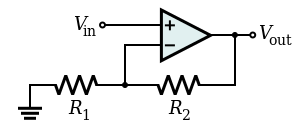
\includegraphics[width=.8\linewidth]{opAmp_nonInverting}
        \captionof{figure}{Non-Inverting Amplifier \cite{opAmpConfigurations}}
        \label{fig:opamp-non-inverting}
    \end{minipage}
    \begin{minipage}{.23\textwidth}
        \centering
        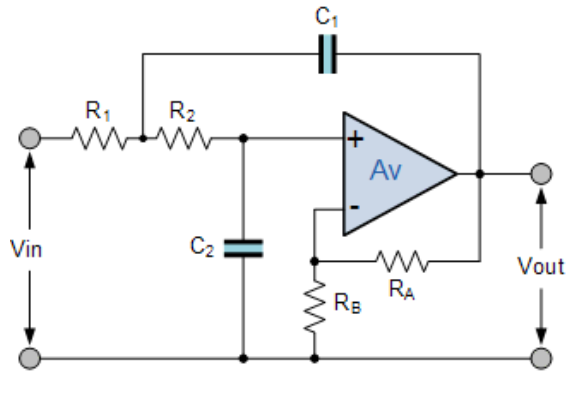
\includegraphics[width=0.8\linewidth]{opAmp_nonInverting_modified}
        \captionof{figure}{Modified Non-Inverting Amplifier \cite{opAmpSecondOrderFilters}}
        \label{fig:opamp-non-inverting-filter}
    \end{minipage}        
    \begin{minipage}{.23\textwidth}
        \centering
        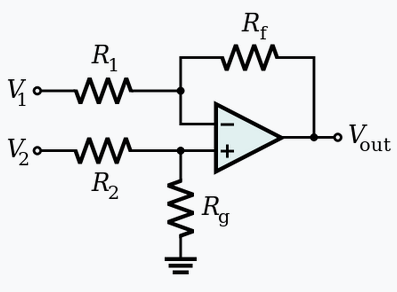
\includegraphics[width=.8\linewidth]{opAmp_differential}
        \captionof{figure}{Differential Amplifier \cite{opAmpConfigurations}}
        \label{fig:opamp-differential}
    \end{minipage}
    \begin{minipage}{.23\textwidth}
        \centering
        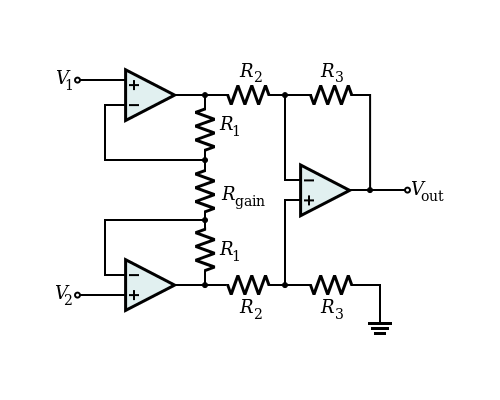
\includegraphics[width=0.9\linewidth]{opAmp_instrumentation}
        \captionof{figure}{Instrumentation Amplifier \cite{opAmpConfigurations}}
        \label{fig:opamp-instrumentation}
    \end{minipage}

\end{figure}

\pagebreak
\graphicspath{{content/1_literatureReview/figures/}}
\section{Current Sensing}

\subsection{Techniques}
Measurement techniques are usually either "invasive" or "non-invasive". Invasive techniques need to be built into the circuit directly and can have a significant affect
on its operation, whereas non-invasive techniques may be added after the initial circuit design e.g. by measurement of a conductor's magnetic field.
A list of a few of these techniques \cite{currentSenseMethods} include:
\begin{itemize}
    \item A current-sensing resistor in series, which uses Ohm's law with a voltage measurement to calculate current.
    \item Hall element sensors, which measure the potential difference created as a result of the main current's magnetic field bending another current left/right.
    \item Direct coil techniques, which make using of Faraday's law.
\end{itemize}

\begin{figure}[h!]
    \centering
    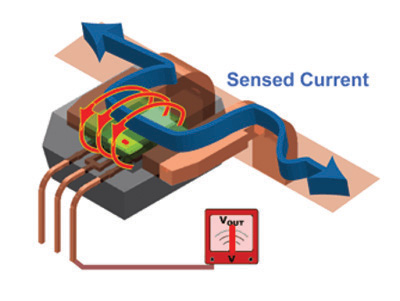
\includegraphics[width=.3\linewidth]{currentSensing_hall_effect}
    \captionof{figure}{Hall Effect Sensor Working Principle \cite{currentSenseHallEffect}}
    \label{fig:hall-effect}
  \end{figure}

\subsection{High-Side vs Low-Side}
This distinction refers to the placement of a current-sense element (e.g. resistor) relative to the load. For circuits which draw higher currents, high-side sensing can be used
(placing the resistor closer to the positive side of the voltage source) and is often more convenient. Low-side sensing, on the other hand, can potentially cause ground loop
issues \cite{currentSenseLowHighSide}, but has the ability to detect faults (e.g. short-circuits) earlier.

\subsection{AC, DC and Power Requirements}
As mentioned, there are various non-invasive and even wireless techniques used to measure current. Coil techniques make use of induction and therefore require AC to operate.
The Hall effect and sense resistors, on the other hand, may be used in the DC case. Wireless techniques have benefits over resistors in that they can be configured to draw much less power,
whereas sense resistors usually require high power handling capabilities as they pass all current drawn by the actual load through them.

\graphicspath{{content/1_literatureReview/figures/}}
\section{Ultrasonic Sensor Interface}\label{sec:ultrasonicSensorInterface}

The HC-SR04 ultrasonic ranging module will be used. It has 4 pins, namely \textit{$V_{cc}$, GND, Trig (Trigger)} and \textit{Echo}.
It should be powered with 5 ${V_{dc}}$ and requires at least 15 mA to function, meaning it will dissipate 75 mW of power. 
First, \textit{Trig} should be pulled high to indicate that the device should send a burst of ultrasonic sound out.
Then, if the sound wave is received back, the device will output a distance-proportional pulse on the \textit{Echo} pin.

\begin{figure}[!htb]
  \centering
  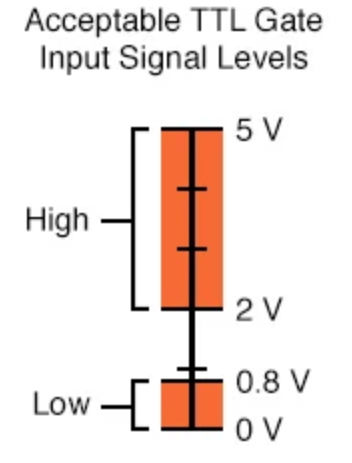
\includegraphics[width=0.15\textwidth]{sonicSensor_TTL}
  \caption{TTL Input/Output Levels \cite{ttlLevels}}
  \label{fig:sonicSensor_TTL}
\end{figure}

The following detailed procedure should be followed to make a distance measurement \cite{datasheetHCSR04}, as also indicated in Figure \ref{fig:sonicSensor_timing}:
\begin{enumerate}
    \item A pulse of at least \SI{10}{\micro\second} should be output onto \textit{Trig}. This pulse must be TTL compliant as indicated
    in Figure \ref{fig:sonicSensor_TTL} i.e. between 2 and 5 V.
    \item If the sound wave is received back by the sensor, \textit{Echo} (also TTL) will go high for ${t_{high}}$ seconds, where ${t_{high}}$ is the time it took the wave to return to the sensor.
          This signal should therefore be conditioned if a circuit which requires 3.3 V is used.
    \item The distance can then be calculated. One of the following methods may be used:
    \begin{enumerate}
        \item The length of time of the \textit{Echo} output signal can be digitally measured and the distance then calculated using \inlineequation[eqn:sensor_distanceFormula]{Distance = \frac{t_{high} * v_{sound}}{2}} \cite{datasheetHCSR04}.
        \item The output pulse can be converted to an analog signal using filtering. The resultant filtered voltage will also be proportional to $t_{high}$.
    \end{enumerate}
    \item A minimum of 60 ms should be present in between each pulse. This allows for a theoretical range of $\frac{\SI{60}{\milli\second} * \SI{340}{m.s^{-1}}}{2} = \SI{10.2}{\metre}$.
          In practice, the device has a range of $\approx 4 m$.
\end{enumerate}

\begin{figure}[!htb]
  \centering
  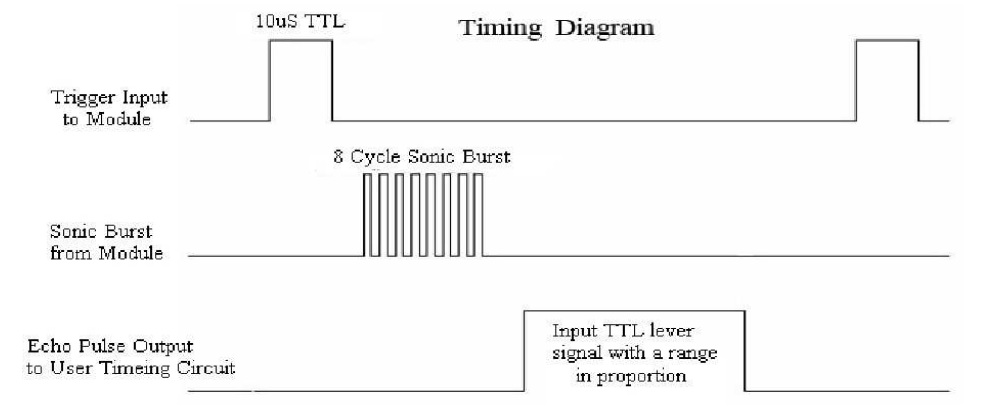
\includegraphics[width=0.5\textwidth]{sonicSensor_timing}
  \caption{Sensor timing diagram \cite{datasheetHCSR04}}
  \label{fig:sonicSensor_timing}
\end{figure}
\graphicspath{{content/1_literatureReview/figures/}}
\section{PWM to Analog Conversion}\label{sec:pwmAnalogConversion}

PWM (Pulse Width Modulation) is useful in that it allows analog information to be conveyed in digital signals.
PWM waves are similar to square waves, however differ in that $t_{high} \neq t_{low}$. A PWM signal is defined by 3 properties:
\begin{itemize}
    \item Frequency: The rate at which the signal oscillates. $f = \frac{1}{t_{high} + t_{low}}$ Hz.
    \item Amplitude: The difference between "high" and "low" voltages. $A = V_{high} - V_{low}$ V.
    \item Duty cycle: The ratio of the signal's "high time" to its period. $\tau = \frac{t_{high}}{t_{high} + t_{low}}$ s.
\end{itemize}

\begin{figure}[!htb]
  \centering
  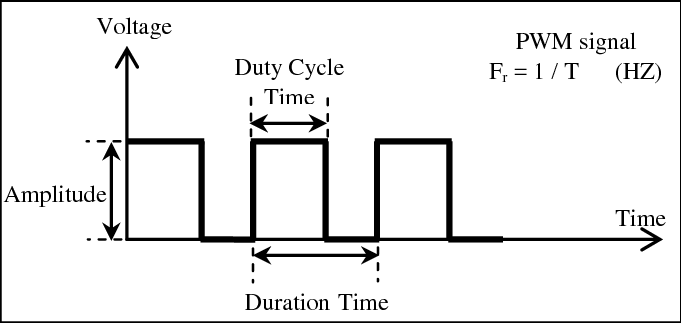
\includegraphics[width=0.25\textwidth]{pwm_graph}
  \caption{PWM Signal Voltage vs Time \cite{pwmGraph}}
\end{figure}

Often, this analog information is conveyed in a varying duty cycle ($\tau$). To convert this varying value to analog,
a low-pass filter can be used. Since the signal's average value increases with $\tau$, filtering out all "harmonics" of the
signal will result in \inlineequation[eqn:pwm_filtered_amplitude]{V_{out} = A \times \tau} \cite{pwmAnalogConversion}. The cutoff frequency ($f_{c}$) of the filter
should be as low as possible, while maintaining an acceptable rise time, in order to minimize ripple on the filter output.
Then, since $t_r \propto \frac{1}{f_c}$, $t_{r(max)}$ will determine the minimum cutoff frequency, $f_{c(min)}$. This will be based on the filter used
e.g. $f_{c(min)}$ = $\frac{3.3}{2 \pi \cdot t_{r(max)}}$ for a \nth{2} order filter [\ref{filter_formulae}].

\begin{figure}[!htb]
  \centering
  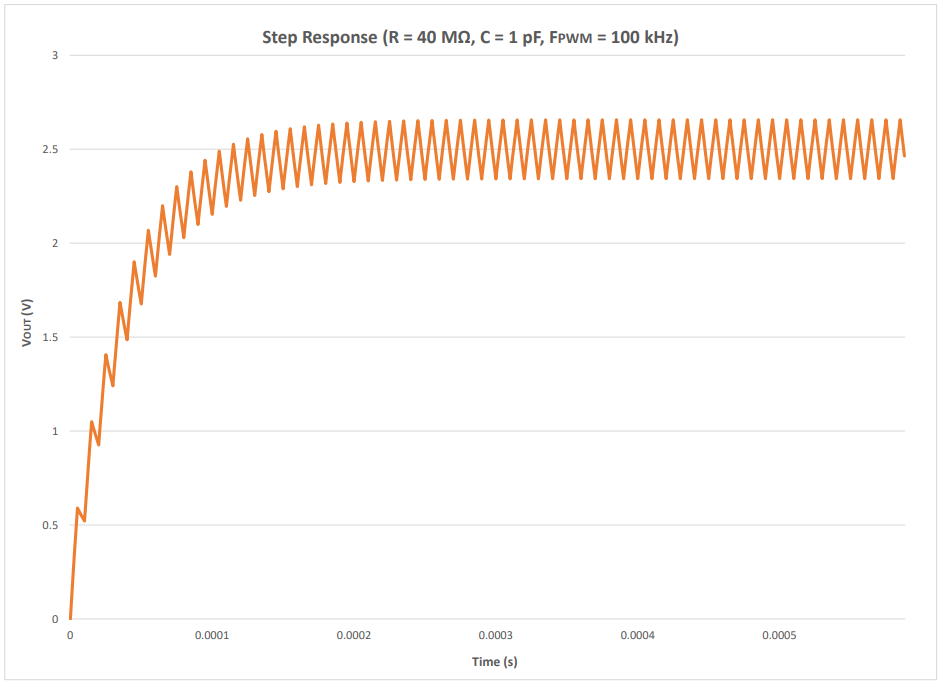
\includegraphics[width=0.3\textwidth]{pwm_filtered}
  \caption{Filtered PWM signal}
\end{figure}

Assuming $f_{c(min)}$ is fixed, $f_{c(max)}$ should be determined by the maximum acceptable noise on the output of the filter.
Since filtering will still leave a small "ripple" signal at frequency $f_{PWM}$, this will be the largest noise component. Given the following:
\begin{itemize}
  \item $A$: Amplitude of the PWM signal (V)
  \item $\tau_{max}$: Maximum duty cycle of the PWM signal (\%)
  \item $N_{max}$: Maximum acceptable noise of the filtered output (V)
\end{itemize}

\noindent Then the required attenuation at $f_{PWM}$ is given by \inlineequation[eqn:pwm_required_attenuation]{A_{dB} = 20 \log \left[ \frac{A \cdot \tau_{max}}{N_{max}} \right]}.
This will determine $f_{c(max)}$, in conjunction with the type of filter used and its order.
\input{content/1_literatureReview/ultrasonicSensorFundamentals}
\graphicspath{{content/2_design/figures/}}
\section{DAC}
\subsection{Configuration and Impedance}

The inverting, R2R configuration will be used. The benefit of a virtual ground, high input impedance,
and low component count are some reasons for this. A voltage divider will be added at $V^+$ to offset the negative gain,
and a buffer stage will be used for better output current.
The ESP32 pin output impedance is typically $30 - \SI{40}{\ohm}$ \cite{datasheetESP}. In order to have less than 1\% deviation of ESP voltage, we can solve for $R_{in}$ using:
$$\frac{V_{cc} - V_{pin}}{V_{cc}} = \frac{R_{in}}{R_{in} + R_{ESP}} \leq 0.01 \therefore R_{in} \geq \SI{3.5}{\kilo\ohm} $$

\noindent The output impedance of the MCP is $R_o \approx \frac{\SI{5.5}{V}}{\SI{23}{mA}} = \SI{239}{\ohm}$ \cite{datasheetMCP6242}. The MCP also has current
protection, and can continuously source/sink $\SI{23}{mA}$ to a $\SI{0}{ohm}$ load. The buffer stage will decouple the negative feedback loop of the summer
from the load stage, adding protection.

\subsection{Amplifier}

All ESP pins are either 0 or 3.3 V. An amplifier current limit of $\SI{250}{\micro\ampere}$ (after quiescent current),
and a pin limit of $\SI{50}{\micro\ampere}$ per digital input is chosen. Since an inverting configuration with a virtual ground (which will be $<< \SI{3.6}{V}$) has been used,
the common-mode range of the op-amp is not violated. Since the MCP can only reach within 35 mV of the rails, an output range of $\SI{0.1}{V} < V_{out} < \SI{3.1}{V}$ will be designed for.
Both stages can be powered by 5 V.
\begin{itemize}
    \item For amplifier current, $R_f > \frac{\SI{3.3}{V}}{\SI{250}{\micro\ampere}} = \SI{13.2}{\kilo\ohm}$.
          For input current, $2R > \frac{\SI{3.3}{V}}{\SI{50}{\micro\ampere}} = \SI{66}{\kilo\ohm}$. 
    \item Choose $2R = \SI{100}{\kilo\ohm}$. For 1111, and using the summing amplifier formula (before offset),
          $V_{out} = \SI{-3}{V} = -\left[ \frac{R_f}{2R} \times 3.3 + \frac{R_f}{4R} \times 3.3 + \frac{R_f}{8R} \times 3.3 + \frac{R_f}{16R} \times 3.3 \right]$
          $\therefore R_f = \SI{48.485}{\kilo\ohm}$. Choose $R_f = \SI{47}{\kilo\ohm} + \SI{4.7}{\kilo\ohm}$pot.
    \item For $V_{out} = \SI{3.1}{V}$ with 0000 input, $V^+ = V^- = \SI{3.1}{V} \times \frac{\SI{50}{\kilo\ohm}}{\SI{48.485}{\kilo\ohm} + \SI{50}{\kilo\ohm}} \approx \SI{1.574}{V}$.
          For the voltage divider, choose $R_a = \SI{47}{\kilo\ohm} \therefore R_b = \SI{21.59}{\kilo\ohm}$. Choose $R_b = \SI{18}{\kilo\ohm} + \SI{10}{\kilo\ohm}$pot.
\end{itemize}

\begin{figure}[!htb]
  \centering
  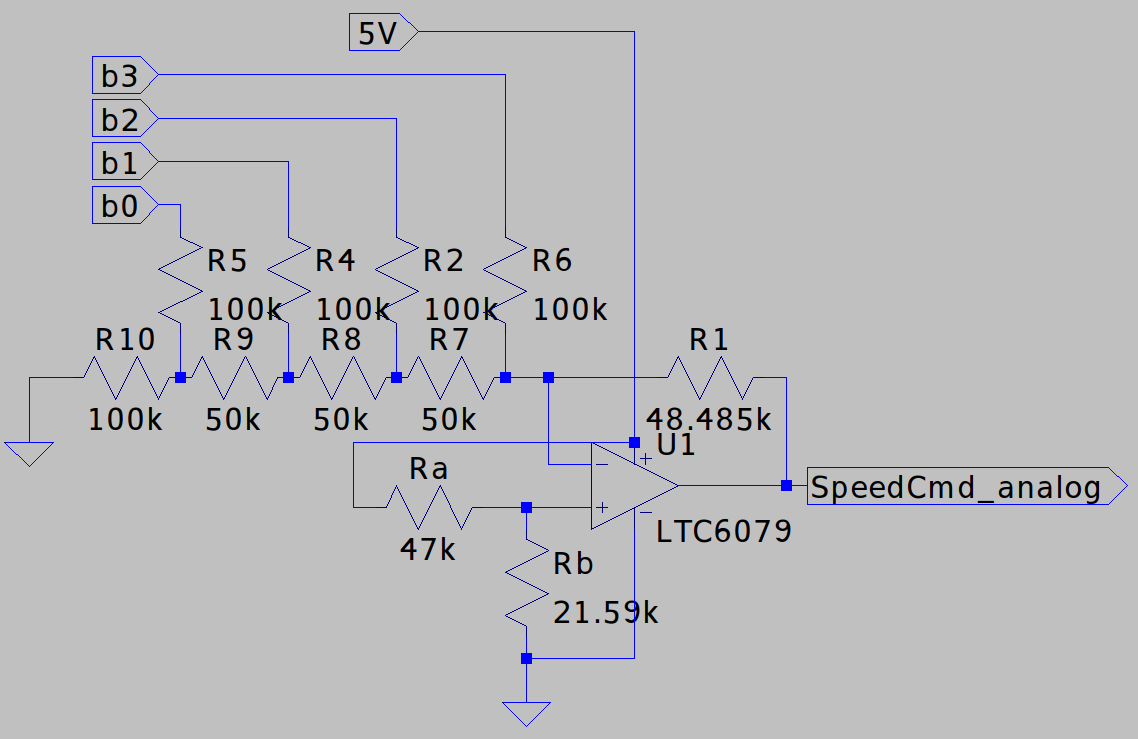
\includegraphics[width=0.42\textwidth]{dac_circuitDiagram}
  \caption{Final Circuit Diagram}
  \label{fig:dac_circuitDiagram}
\end{figure}
\graphicspath{{content/figures/}}
\chapter{Detailed Design}

\graphicspath{{content/2_design/figures}}

\section{System Design}

The final block diagram for the system can be found in Figure \ref{fig:voltageRegulation_blockDiagram}.

\begin{figure}[!htb]
  \centering
  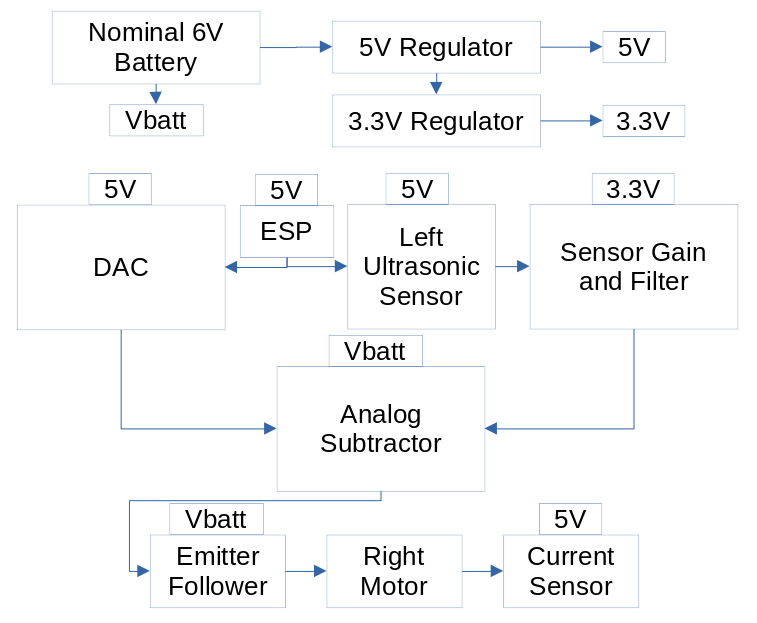
\includegraphics[width=0.8\textwidth]{voltageRegulation_blockDiagram}
  \caption{Final System Block Diagram}
  \label{fig:voltageRegulation_blockDiagram}
\end{figure}

\pagebreak
\graphicspath{{content/2_design/figures}}

\section{Voltage Regulation}

The LD1117V and LD33CV will be used for 5 V and 3.3 V regulation respectively. The circuit diagram for both circuits is shown in the figures below.
The LD33CV has a maximum dropout voltage of 1.3 V \cite{datasheetLD1117}. This means that it can safely be powered directly from the 5 V regulator, as 5 V - 1.3 V = 3.7 V.
The variable LD1117V also has a maximum dropout voltage of 1.3 V \cite{datasheetLD1117}, and can handle an input operating voltage of maximum 15 V. This means it can safely be
powered from the maximum 7.2 V battery supply, however will suffer when the supply drops below $\SI{6.3}{V}$. Under-voltage protection should therefore be implemented.

\begin{figure}[!htb]
    \centering
    \begin{minipage}{.4\textwidth}
        \centering
        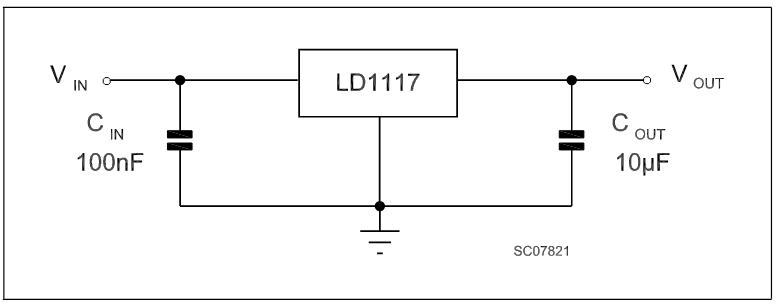
\includegraphics[width=1.0\linewidth]{voltageRegulation_3v3}
        \captionof{figure}{3.3 V Circuit \cite{datasheetLD1117}}
        \label{fig:voltageRegulation_3v3}
    \end{minipage}
    \begin{minipage}{.4\textwidth}
        \centering
        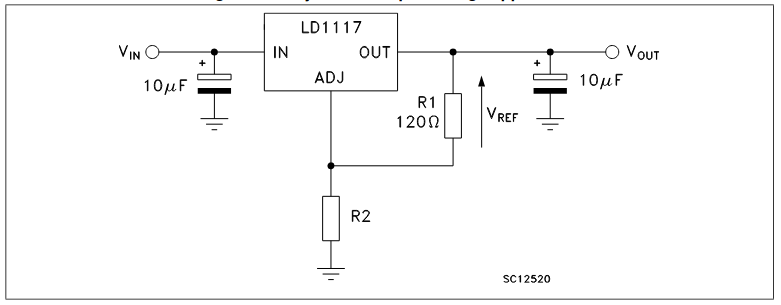
\includegraphics[width=1.0\linewidth]{voltageRegulation_5v}
        \captionof{figure}{5 V Circuit \cite{datasheetLD1117}}
        \label{fig:voltageRegulation_5v}
    \end{minipage}
\end{figure}

The feedback resistor values simply need to be calculated. According to \cite{datasheetLD1117}, $R_2$ in Figure \ref{fig:voltageRegulation_5v}
can be calculated using $V_{out} = V_{ref} (1 + \frac{R2}{R1})$. With $V_{out} = \SI{5}{V}$, $V_{ref} \approx \SI{1.25}{V}$, and $R_1 = \SI{120}{\ohm}$,
$R_2 = R_1 \cdot \left(\frac{V_{out}}{V_{ref}} - 1\right) = \SI{360}{\ohm}$. A $\SI{470}{\ohm}$ potentiometer will be used for the practical circuit to adjust the output to exactly $\SI{5}{V}$.

\pagebreak
\graphicspath{{content/4_implementation/figures/}}
\section{Current sensor}\label{sec:current_sensor_physical}

The implementation of the circuit was different in two ways compared to the original design:
\begin{itemize}
   \item \SI{120}{\kilo\ohm} resistors were used instead of \SI{100}{\kilo\ohm}, as they were easier to obtain, and would only result in a
         slightly larger gain and lower cutoff.
   \item The amplifier circuit was powered with regulated \SI{3.3}{V}. This was done to protect the ESP's input pins by saturating the output
         when it would have been too large.
\end{itemize}

\begin{figure}[!htb]
  \centering
  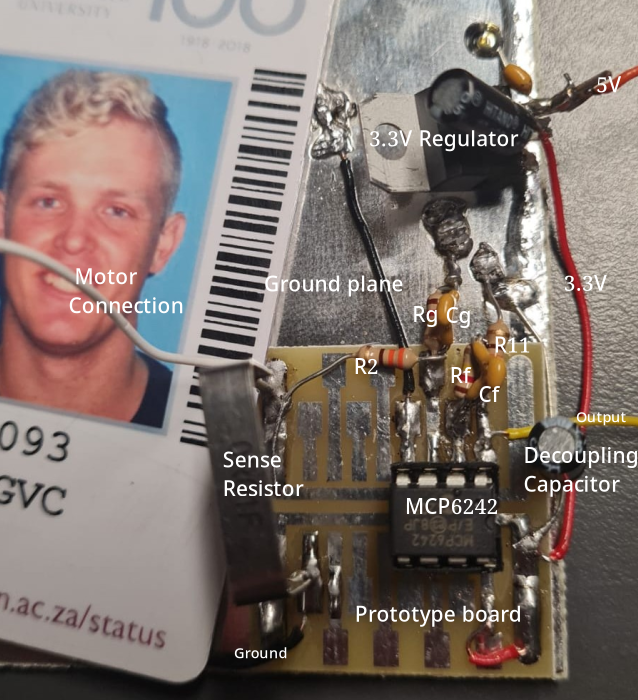
\includegraphics[width=0.75\textwidth]{currentSensor_impl_circuit}
  \caption{Final Circuit Implementation}
\end{figure}
\graphicspath{{content/2_design/figures/}}
\section{Ultrasonic Sensor}
\subsection{Power and Output Requirements}
The range sensor requires \SI{5}{V_{dc}} power and will draw around \SI{15}{mA}. Since the LD1117V provides a stable 5.0 V output and is capable
of providing up to 800 mA of current, the sensor will be powered directly from this regulator.

The sensor's echo output is a PWM wave of varying duty cycle $\tau$ and $f_{PWM} = \SI{16}{Hz}$.
This signal's amplitude could be as high as 5 V (TTL level). The maximum output $A_{max}$ \textit{after} unity filtering,
however, will be determined by the maximum duty cycle, $t_{max}$. Since a distance of $D_{max} = \SI{1}{m}$ and $D_{min} = \SI{5}{cm}$,
Equations \ref{eqn:sensor_distanceFormula} and \ref{eqn:pwm_filtered_amplitude} can be used to calculate:
\begin{itemize}
  \item At $D_{max}$, $t_{max} \approx \SI{5.9}{ms}$, $\tau_{max} = \frac{\SI{5.9}{ms}}{1/16} \approx 9.5 \%$ and $A_{max} = (\SI{5}{V}) \cdot (9.5 \%) = \SI{475}{mV} $.
  \item At $D_{min}$, $t_{min} \approx \SI{0.29}{ms}$, $\tau_{min} = \frac{\SI{0.29}{ms}}{1/16} \approx 0.47 \%$ and $A_{min} = (\SI{5}{V}) \cdot (0.47 \%) = \SI{23}{mV} $.
\end{itemize}

\subsection{Filter Selection}{\label{rangeSensor_filterSelection}}

To determine the filter's order, rise time and noise requirements should be considered:
\begin{itemize}
  \item After filtering, since gain $\approx \frac{\SI{3}{V}}{\SI{475}{mV}} \approx \SI{7}{V/V}$, filter ripple must be under $ \frac{\SI{70}{mV}}{7} = \SI{7}{mV}$.
  \item A 10\% to 90\% rise time ($t_r$) of \SI{1.5}{s} should be adhered to.
\end{itemize}

\noindent These specifications result in the requirement that $A_{dB}$ at $f_{PWM} = 20 \log \left[ \frac{\SI{5}{V}}{\SI{7}{mV}} \right] \approx \SI{60}{dB}$.
A \nth{3} order filter with $f_c = \SI{1}{Hz}$ will be used, as a \nth{2} order may be tolerance-sensitive.
This provides $t_r \approx 0.63 s$ and $A_{dB} \approx 72 dB $ [\ref{filter_formulae}].

\begin{table}[!h]
  \centering
  \renewcommand{\arraystretch}{1.2}
  \begin{tabular}{ |c|c|p{2.5cm}|p{2.5cm}|p{3.5cm}| }
    \hline
    \textbf{Filter type}  & \textbf{Design Spec.}         & \textbf{Cutoff $f_c$}     & \textbf{Rise time $t_r$}        & \textbf{Attenuation $A_{dB}$}       \\
    \hline
    \nth{1} order            & Rise Time                     & 0.233 Hz                  & 1.5 s                           & 37 dB                               \\
                             & Attenuation                   & 0.016 Hz                  & 22 s                            & 60 dB                               \\ \hline
    \nth{2} order            & Rise Time                     & 0.350 Hz                  & 1.5 s                           & 66 dB                               \\
                             & Attenuation                   & 0.505 Hz                  & 1.038 s                         & 60 dB                               \\ \hline
    \nth{3} order (cascade)  & Rise Time                     & 0.420 Hz                  & 1.5 s                           & 95 dB                               \\
                             & Attenuation                   & 1.600 Hz                  & 0.394 s                         & 60 dB                               \\ \hline
  \end{tabular}
  \caption{Filter type vs Rise Time and Attenuation using [\ref{filter_formulae}]}
  \label{tab:range_sensor_filter_comparison}
\end{table}

\subsection{Configuration}{\label{rangeSensor_circuitConfig}}

A "two-and-a-half" stage configuration will be used. The first stage is a gain/offset and \nth{1} order filter,
and is placed first in order to amplify the signal above the MCP's 35 mV floor. The second stage is unity-gain \nth{2} order filter.
A non-inverting amplifier will be used for stage 1, and a Sallen-Key topology for stage 2. Since the quiescent current for each op-amp is
$\SI{70}{uA}$ \cite{datasheetMCP6242}, stage 1 \& 2 will be allocated $\SI{400}{\micro\ampere}$ and $\SI{200}{\micro\ampere}$ respectively.

\begin{figure}[!htb]
  \centering
  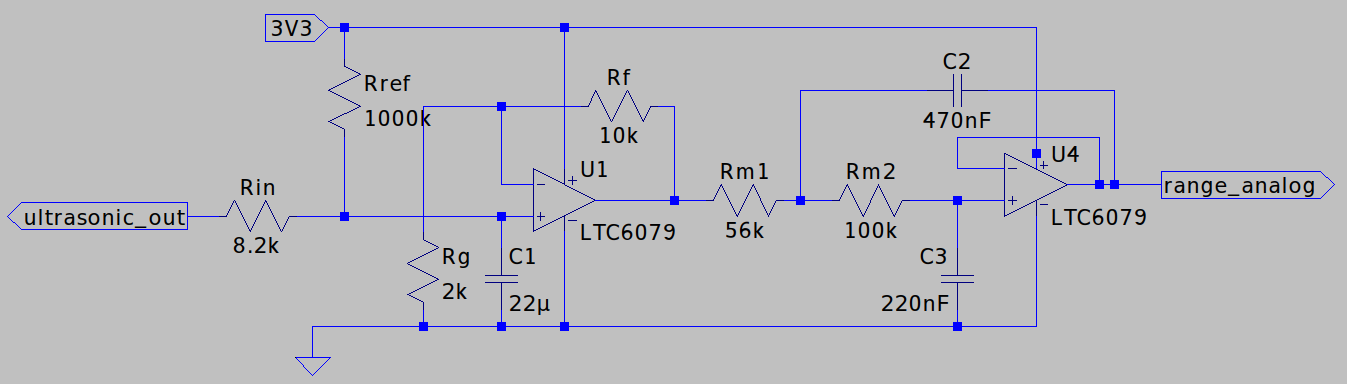
\includegraphics[width=0.8\textwidth]{rangeSensor_circuitDiagram}
  \caption{Range Sensor Amplifier Circuit Diagram}
  \label{fig:rangeSensor_circuitDiagram}
\end{figure}

\subsection{Gain Stage}

This stage will be powered by the 3.3 V regulator. As this is a low-gain circuit, input bias voltages can be neglected.
Slew rate and CMMR imbalance can also be ignored due to the low-frequency, single-ended use of the op-amp.
Voltage rail saturation does not need to be considered at the circuit output, as $\SI{0.3}{V} < V_{out} < \SI{3}{V}$,
and has already been catered for at the input, as discussed in Section \ref{rangeSensor_circuitConfig}.
Using the equations at \cite{gainOffset30Seconds}, and the expected input ranges from the filter stage,
gain $m = \frac{\SI{3}{V} - \SI{0.3}{V}}{\SI{475}{mV} - \SI{23}{mV}} = \SI{5.97}{\volt\per\volt}$,
and offset $b = \SI{0.3}{V} - m \times \SI{23}{mV} \approx \SI{163}{mV}$:

\begin{itemize}
  \item With idle current $I_Q = \frac{V_{out}}{R_f + R_g}$, and $V_{out(max)} = \SI{3.3}{V}$, $(R_f + R_g)_{min} = \frac{\SI{3.3}{V}}{\SI{400}{\micro\ampere}} = \SI{8.25}{\kilo\ohm}$.
  \item Since the offset voltage is low, $R_{ref}$ will be high. A potentiometer will also be used to tune this offset, therefore choose $R_{ref} = \SI{1000}{\kilo\ohm} = \SI{820}{\kilo\ohm} + \SI{470}{\kilo\ohm} \textnormal{pot}$.
  \item Calculate $R_{in} = \frac{R_{ref} \times b}{V_{ref} \times m} \approx \SI{8.2}{\kilo\ohm}$ with $V_{ref} = \SI{5}{V}$ and $C_1 = \frac{1}{2 \pi f_c R_1} \approx \SI{22}{\micro\farad}$.
  \item Choose $R_f = \SI{10}{\kilo\ohm}$ to satisfy the current requirements.
  \item Calculate $R_g = \frac{R_{ref} \times R_f}{m \times (R_{in} + R_{ref}) - R_{ref}} \approx \SI{2}{\kilo\ohm}$. To tune the gain, choose $R_g = \SI{1.5}{k} + \SI{1}{\kilo\ohm}\textnormal{pot}$.
\end{itemize}


\subsection{Filter Stage}

This stage will use the 3.3 V regulator to clip the circuit output for use with the MCU.
This results in the \nth{2} order stage transfer function $H(s) = \frac{1}{1 + 0.2251 s + 0.02533 s^2} = \frac{1}{1 + a_1 s + b_1 s^2}$ with $\zeta = 0.707$. Now, component values can be chosen.
Formulae from \cite{filterDesign} will be used:

\begin{itemize}
  \item Since both capacitors are open-circuit during DC, the idle current is very low. A maximum step input will result in a surge of current through $C_2$ to ground.
        With $V_{in(max)} = \SI{5}{V}$, $(R_{m1} + R_{m2})_{min} = \frac{\SI{5}{V}}{\SI{200}{\micro\ampere}} = \SI{25}{\kilo\ohm}$.
  \item Since $C_3 = \frac{a_1}{2 \pi f_c (R_{m1} + R_{m2})}$ \cite{filterDesign}, choose $C_3 = \SI{220}{nF}$ so that $R_{m1} + R_{m2} \approx \SI{160}{\kilo\ohm}$.
  \item To meet $C_2 \geq C_3 \cdot \frac{4 \cdot b_1}{a_1 ^2} \approx 2 C_3 $ \cite{filterDesign}, choose $C_2 = \SI{470}{nF}$.
  \item Since $C_3 \cdot C_2 = \frac{b_1}{((2 \pi f_c)^2 R_{m1} R_{m2})}$, and $R_{m1} + R_{m2} = \SI{450}{\kilo\ohm}$, solve to obtain $R_{m1} = \SI{61}{\kilo\ohm}$ and $R_{m2} = \SI{99}{\kilo\ohm}$.
        Choose $R_{m1} = \SI{56}{\kilo\ohm}$ and $R_{m2} = \SI{100}{\kilo\ohm}$ as practical values.
\end{itemize}
\graphicspath{{content/3_results/figures}}
\section{Digital to Analog Converter}

\subsection{Simulation}

\begin{figure}[!htb]
    \centering
    \begin{minipage}{.5\textwidth}
        \centering
        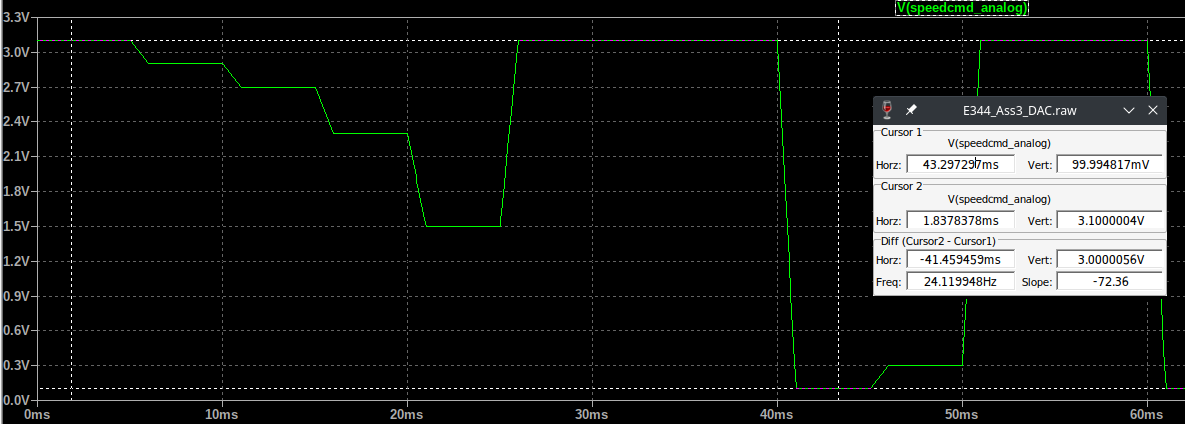
\includegraphics[width=1.0\linewidth]{dac_sim_range}
        \captionof{figure}{Output Range from 0000 (First Cursor) to 1111 (Second Cursor)}
        \label{fig:dac_sim_range}
    \end{minipage}
    \begin{minipage}{.45\textwidth}
        \centering
        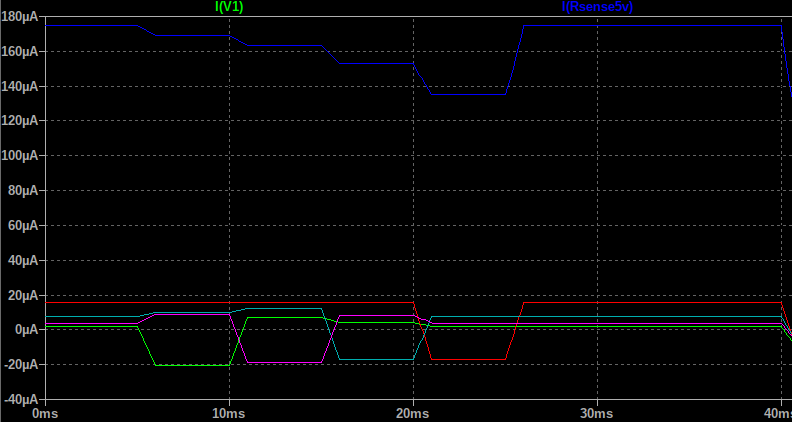
\includegraphics[width=1.0\linewidth]{dac_sim_currentDraw}
        \captionof{figure}{Current Draw (Amplifier and Digital Inputs)}
        \label{fig:dac_sim_currentDraw}
    \end{minipage}
\end{figure}

As seen in the above figures, all specifications were complied with:
\begin{itemize}
    \item Figure \ref{fig:dac_sim_range} shows that an output of 0000 produces exactly 3.1 V on the output, and that 1111 produces 100 mV.
    \item Figure \ref{fig:dac_sim_currentDraw} shows a maximum current draw of under $\SI{180}{\micro\ampere}$, which is much under the $\SI{250}{\micro\ampere}$ specification.
          It also shows that each digital input draws less than $\SI{20}{\micro\ampere}$, also under the $\SI{50}{\micro\ampere}$ specification.
\end{itemize}

\subsection{Implementation}

\begin{figure}[!htb]
    \centering
    \begin{minipage}{.22\textwidth}
        \centering
        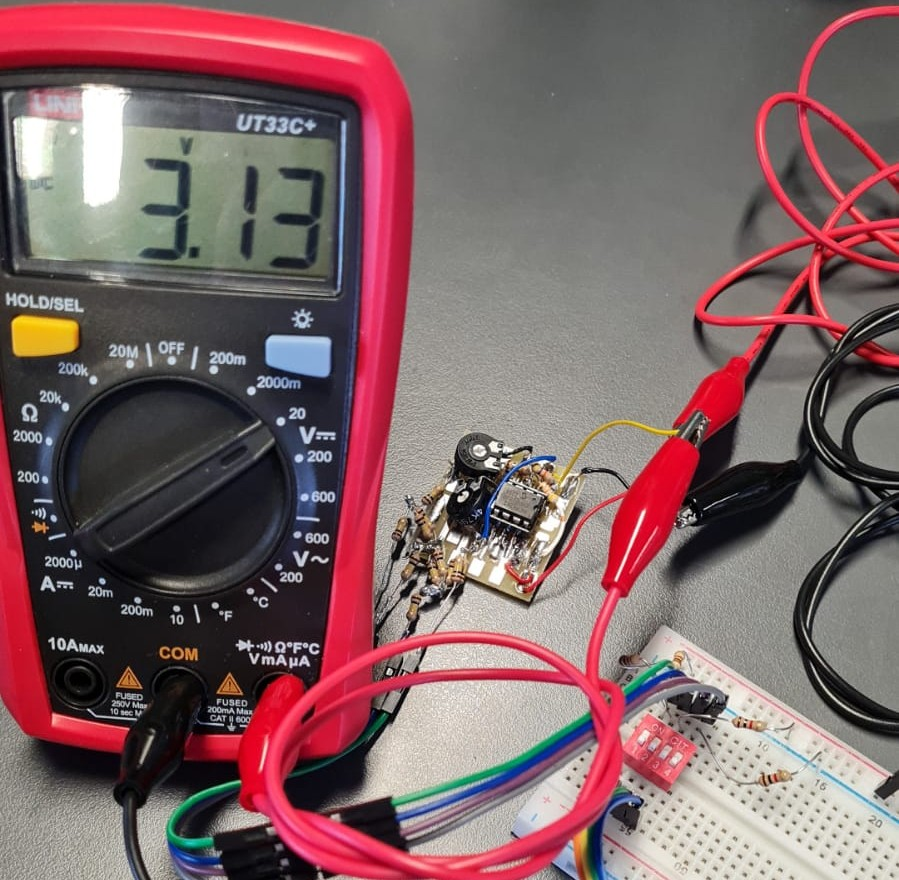
\includegraphics[width=1.0\linewidth]{dac_impl_0000}
        \captionof{figure}{DAC Output at 0000}
        \label{fig:dac_impl_0000}
    \end{minipage}
    \begin{minipage}{.2\textwidth}
        \centering
        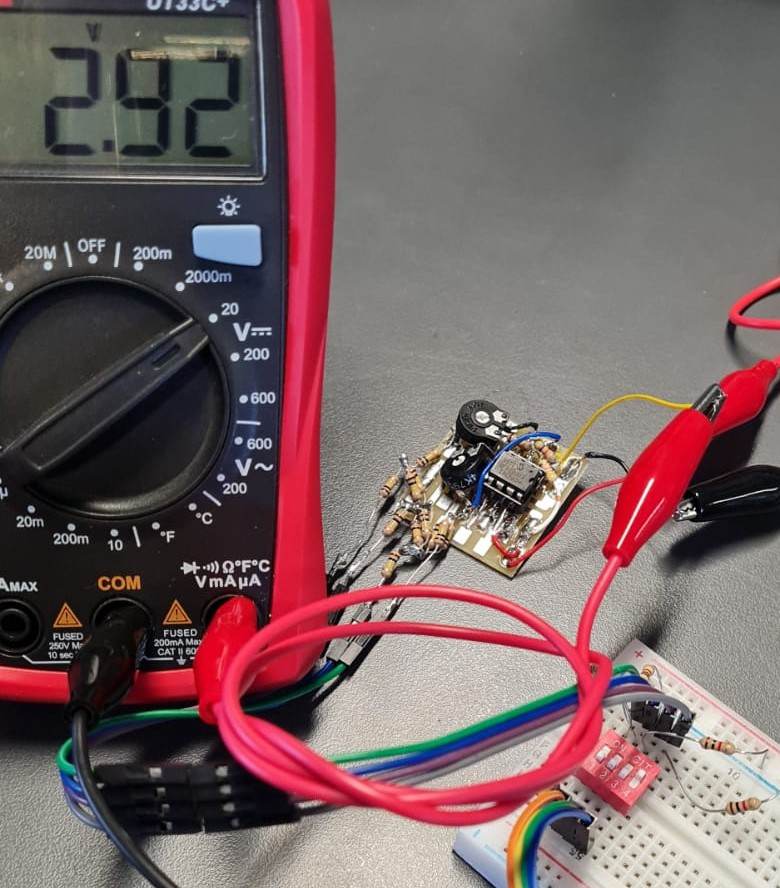
\includegraphics[width=1.0\linewidth]{dac_impl_0001}
        \captionof{figure}{DAC Output at 0001}
        \label{fig:dac_impl_0001}
    \end{minipage}
    \begin{minipage}{.22\textwidth}
        \centering
        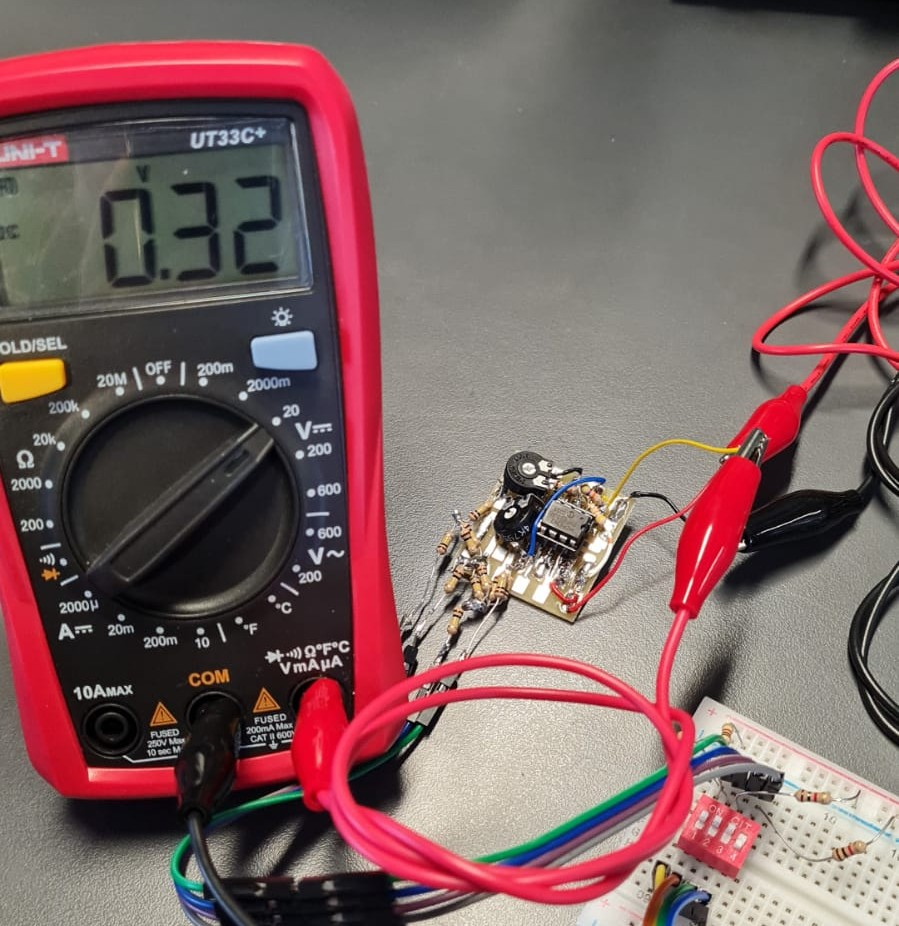
\includegraphics[width=1.0\linewidth]{dac_impl_1110}
        \captionof{figure}{DAC Output at 1110}
        \label{fig:dac_impl_1110}
    \end{minipage}
    \begin{minipage}{.2\textwidth}
        \centering
        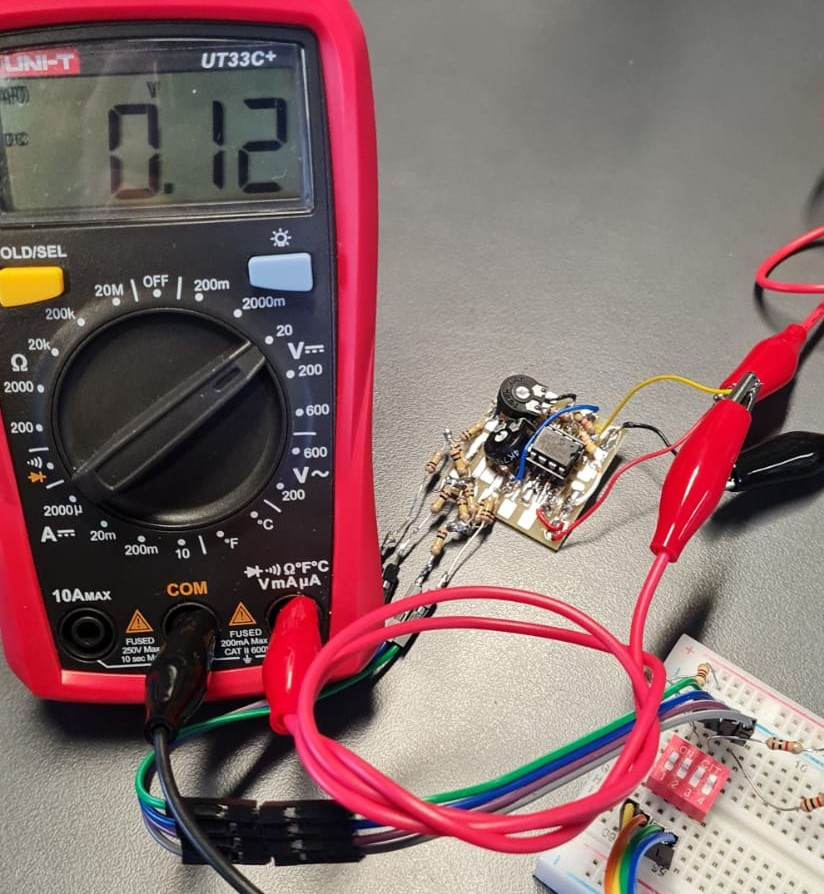
\includegraphics[width=1.0\linewidth]{dac_impl_1111}
        \captionof{figure}{DAC Output at 1111}
        \label{fig:dac_impl_1111}
    \end{minipage}    
\end{figure}

Figures \ref{fig:dac_impl_0000} to \ref{fig:dac_impl_1111} demonstrate the output voltages at specific digital input combinations.
All specifications are complied with, specifically that 0000 produces $> \SI{3}{V}$ on the output, and that 1111 produces $< \SI{0.5}{V}$.
\graphicspath{{content/3_results/figures}}
\section{Analog Motor Controller}

\subsection{Simulated}

The results of the simulation for the two motor controller stages can be found below.

\begin{figure}[!htb]
  \centering
  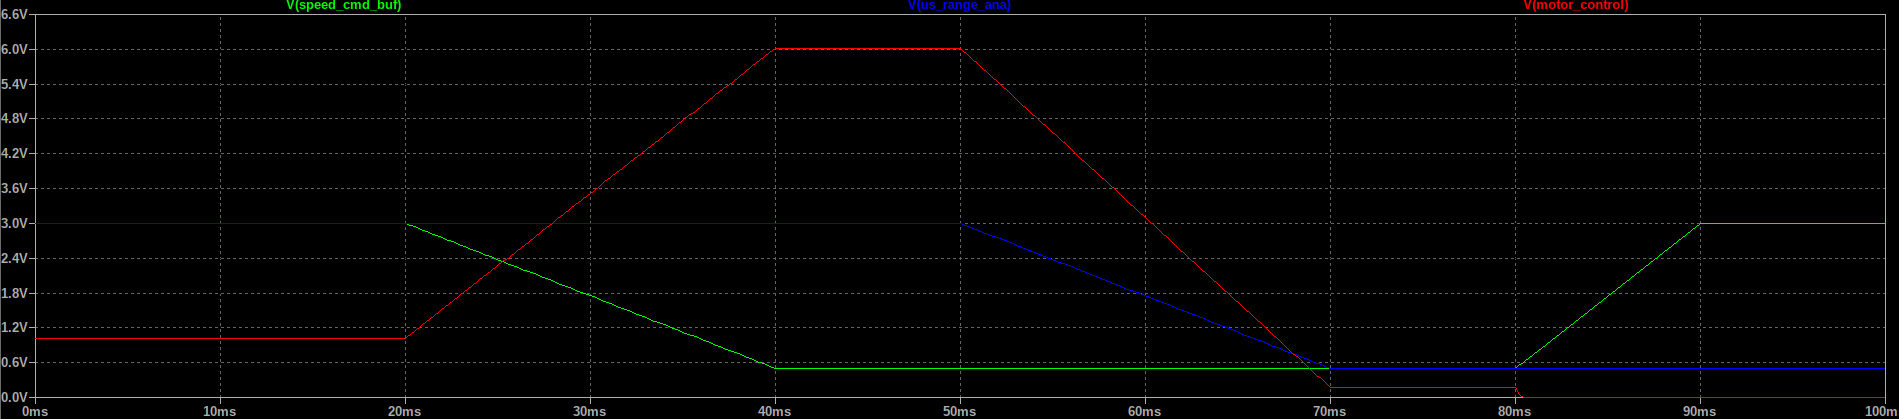
\includegraphics[width=0.8\textwidth]{motorController_sim_subtractor_output}
  \caption{Motor Controller Output of Subtractor Stage}
  \label{fig:motorController_sim_subtractor_output}
\end{figure}

\begin{figure}[!htb]
  \centering
  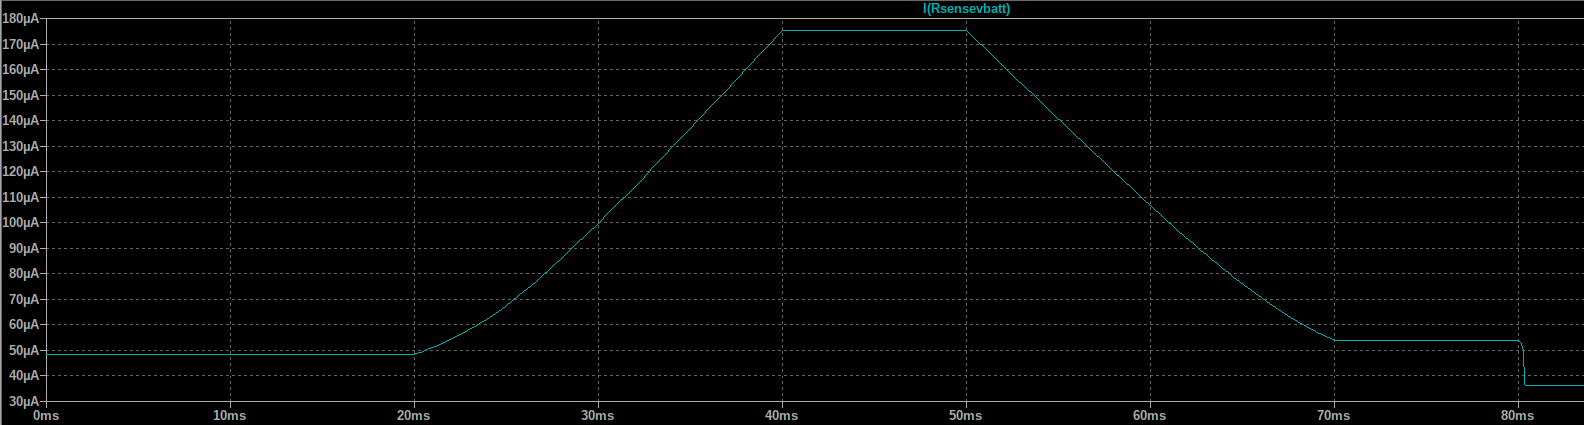
\includegraphics[width=0.6\textwidth]{motorController_sim_subtractor_currentDraw}
  \caption{Motor Controller Current Draw of Subtractor Stage}
  \label{fig:motorController_sim_subtractor_currentDraw}
\end{figure}

\begin{figure}[!htb]
    \centering
    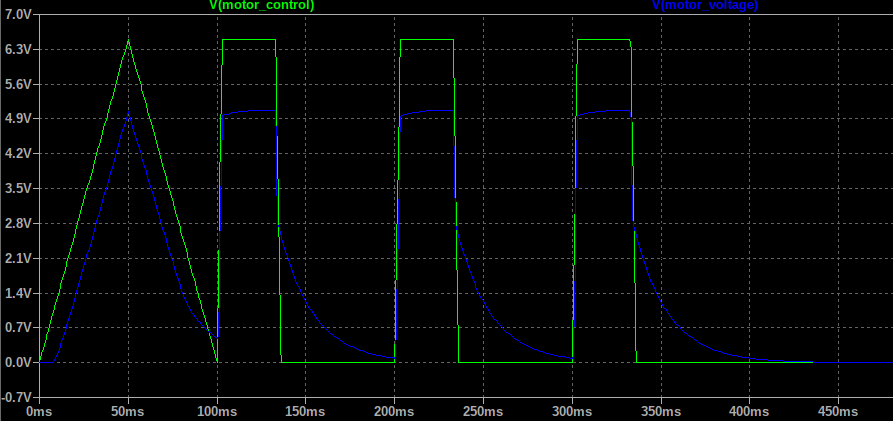
\includegraphics[width=0.45\textwidth]{motorController_sim_power_output}
    \caption{Motor Controller Output of Power Stage}
    \label{fig:motorController_sim_power_output}
  \end{figure}

As can be seen, specifications were complied to:
\begin{itemize}
    \item A "low speed" command (3 V) and "no object" command (3 V) results in a low controller command ($< \SI{1.8}{V}$).
    \item A "high speed" command (0.5 V) and "no object" command (3 V) results in a high controller command. The output, however, only reaches 6 V
          due to a different input range. A simulation with $V_{speed} = \SI{0.1}{V}$ and $V_{range} = \SI{3.3}{V}$ shows that the output saturates at 7.2 V.
    \item The current draw of the subtractor is as designed i.e. $< \SI{400}{\micro\ampere}$, and therefore the total current is $< \SI{1.5}{A}$ due to the
          maximum motor current draw of $\SI{1}{A}$.
    \item The drop from the motor control command to the motor is $\SI{1.4}{V}$, meaning the designed minimum of $\SI{1.8}{V}$ will ensure the motor
          has $V_{motor} < \SI{0.5}{V}$.
\end{itemize}

\subsection{Measured}

Voltage measurements over the motor for the four edge-cases of the motor controller can be seen below.

\begin{figure}[!htb]
    \centering
    \begin{minipage}{.38\textwidth}
        \centering
        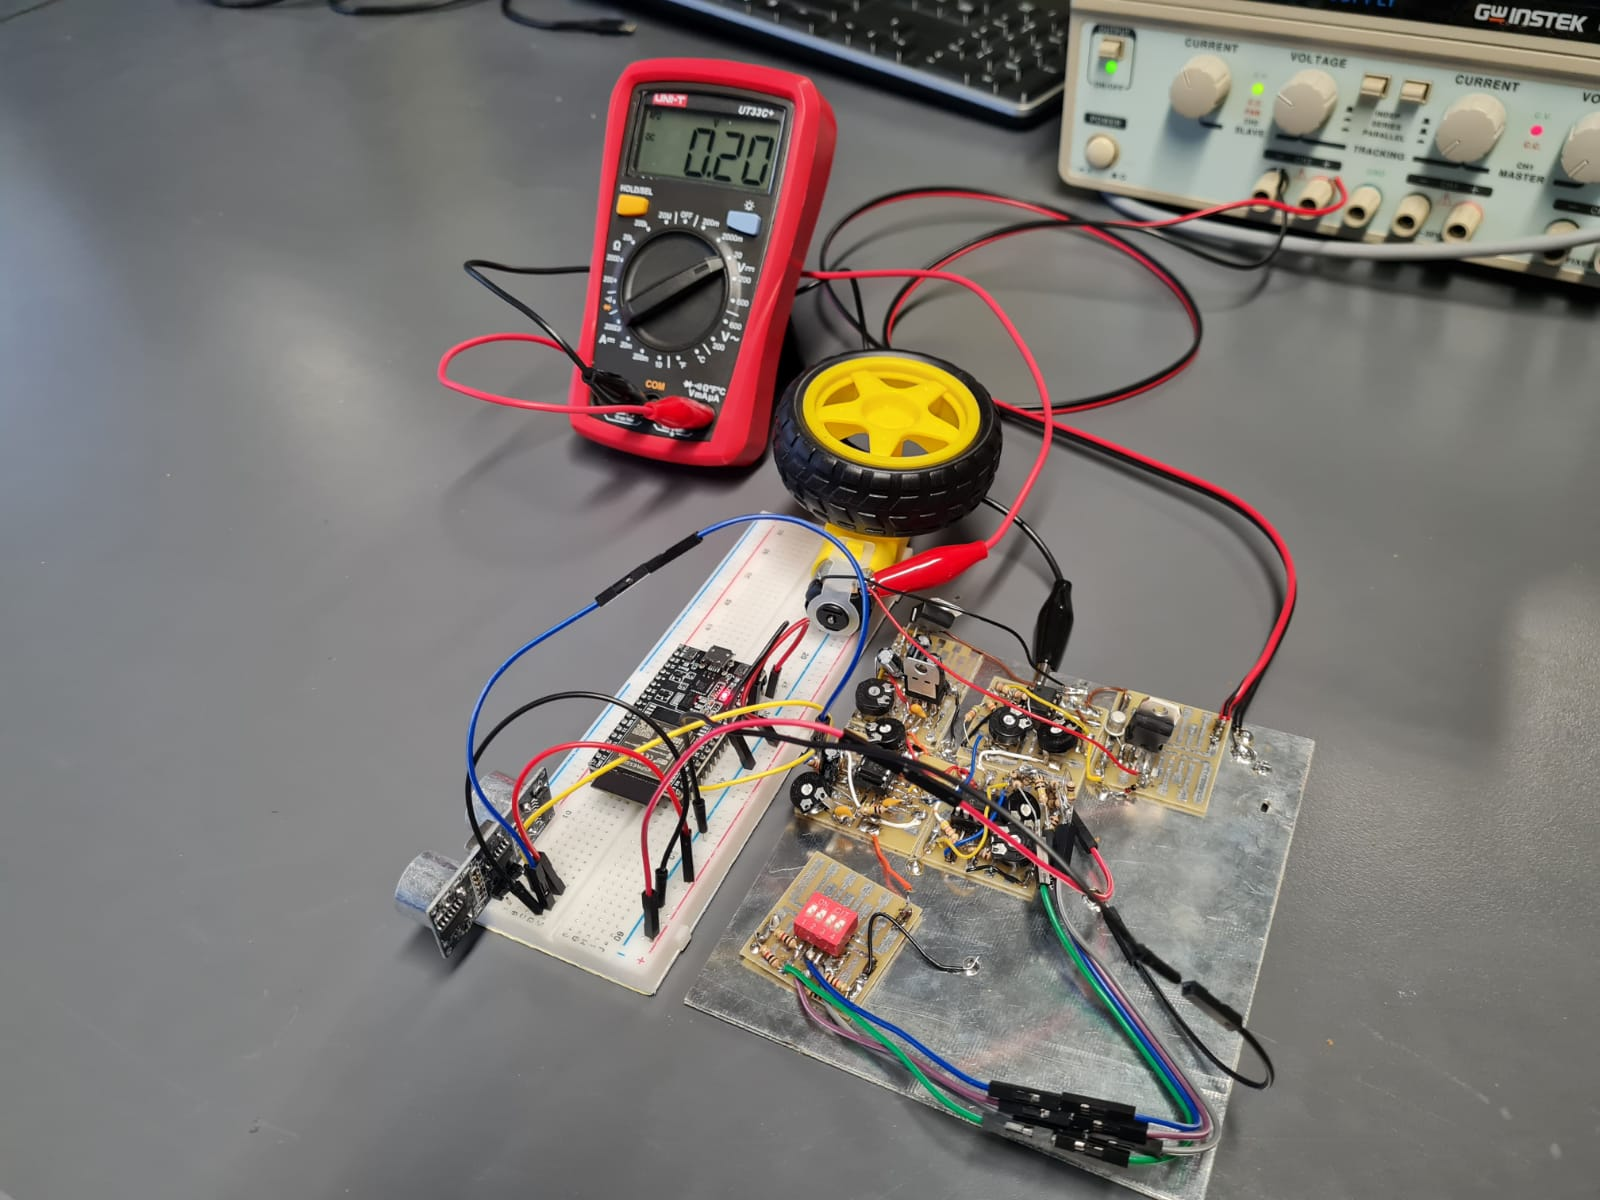
\includegraphics[width=1.0\linewidth]{motorController_far_0000}
        \captionof{figure}{Motor Voltage: Object Far, Speed 0000}
        \label{fig:motorController_far_0000}
    \end{minipage}
    \begin{minipage}{.38\textwidth}
        \centering
        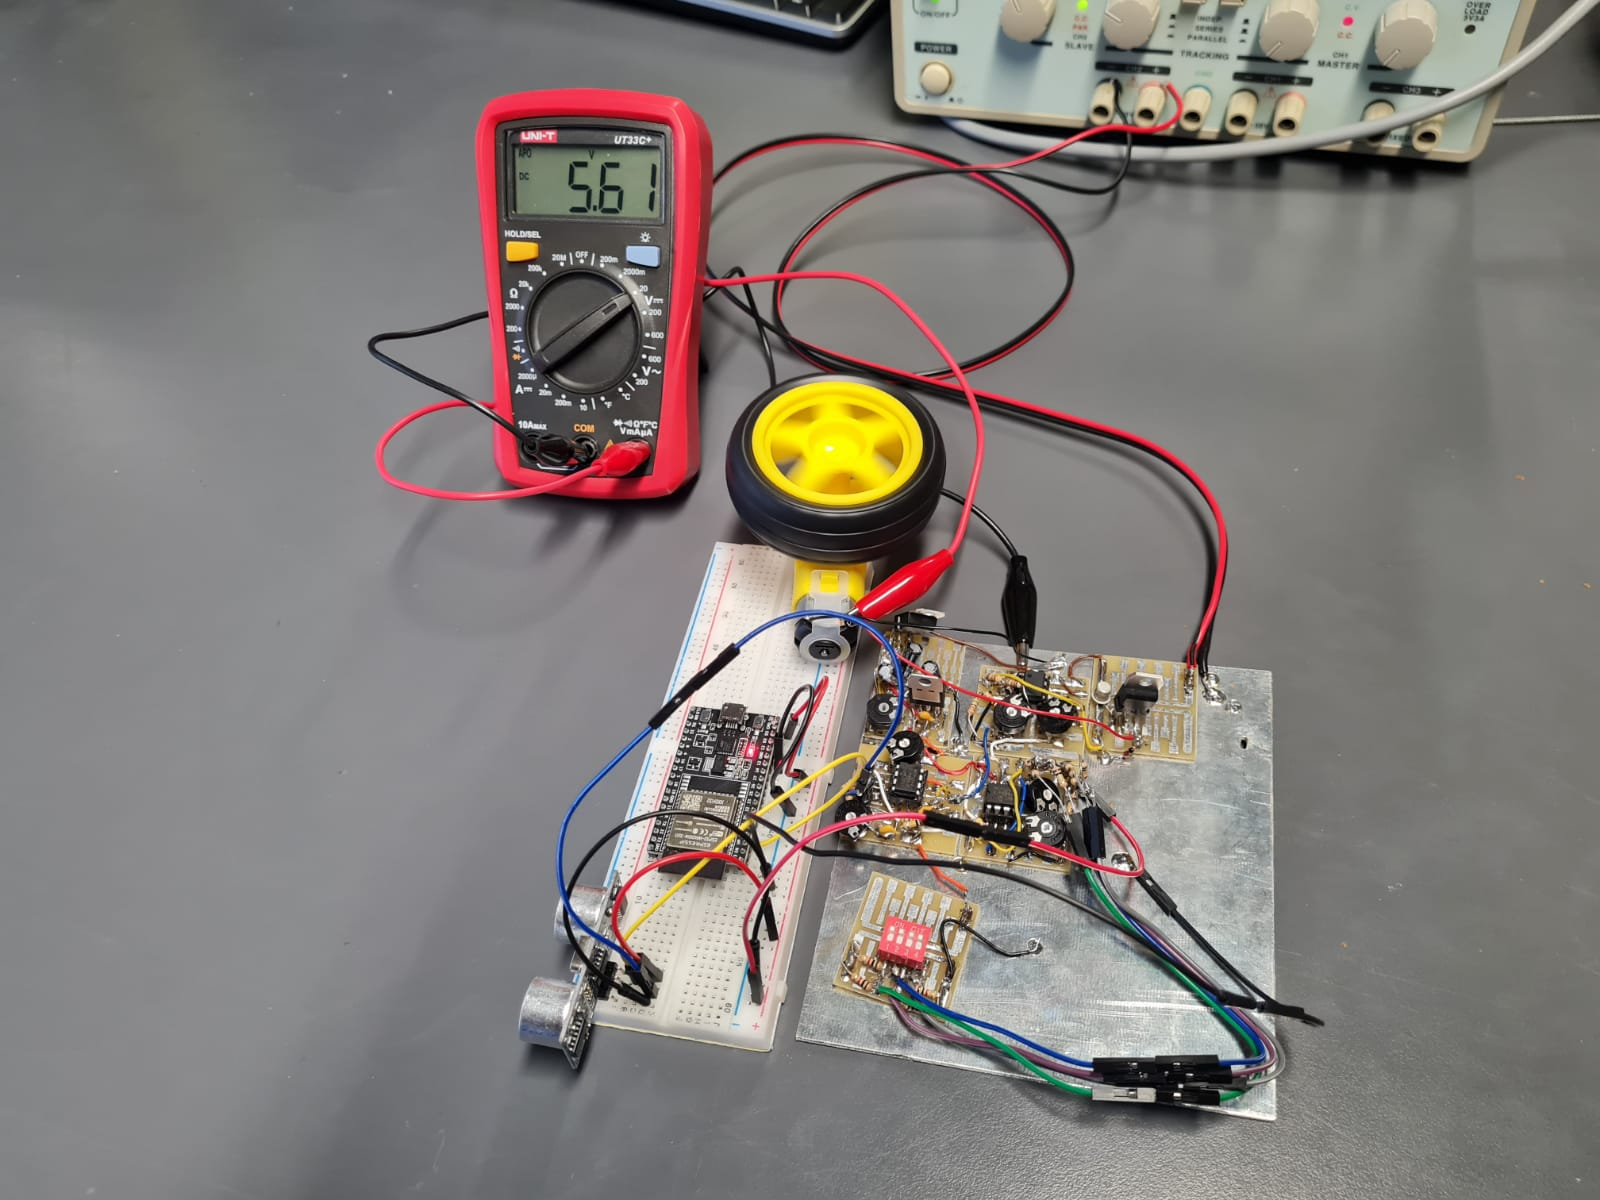
\includegraphics[width=1.0\linewidth]{motorController_far_1111}
        \captionof{figure}{Motor Voltage: Object Far, Speed 1111}
        \label{fig:motorController_far_1111}
    \end{minipage}
\end{figure}

\begin{figure}[!htb]
    \centering
    \begin{minipage}{.38\textwidth}
        \centering
        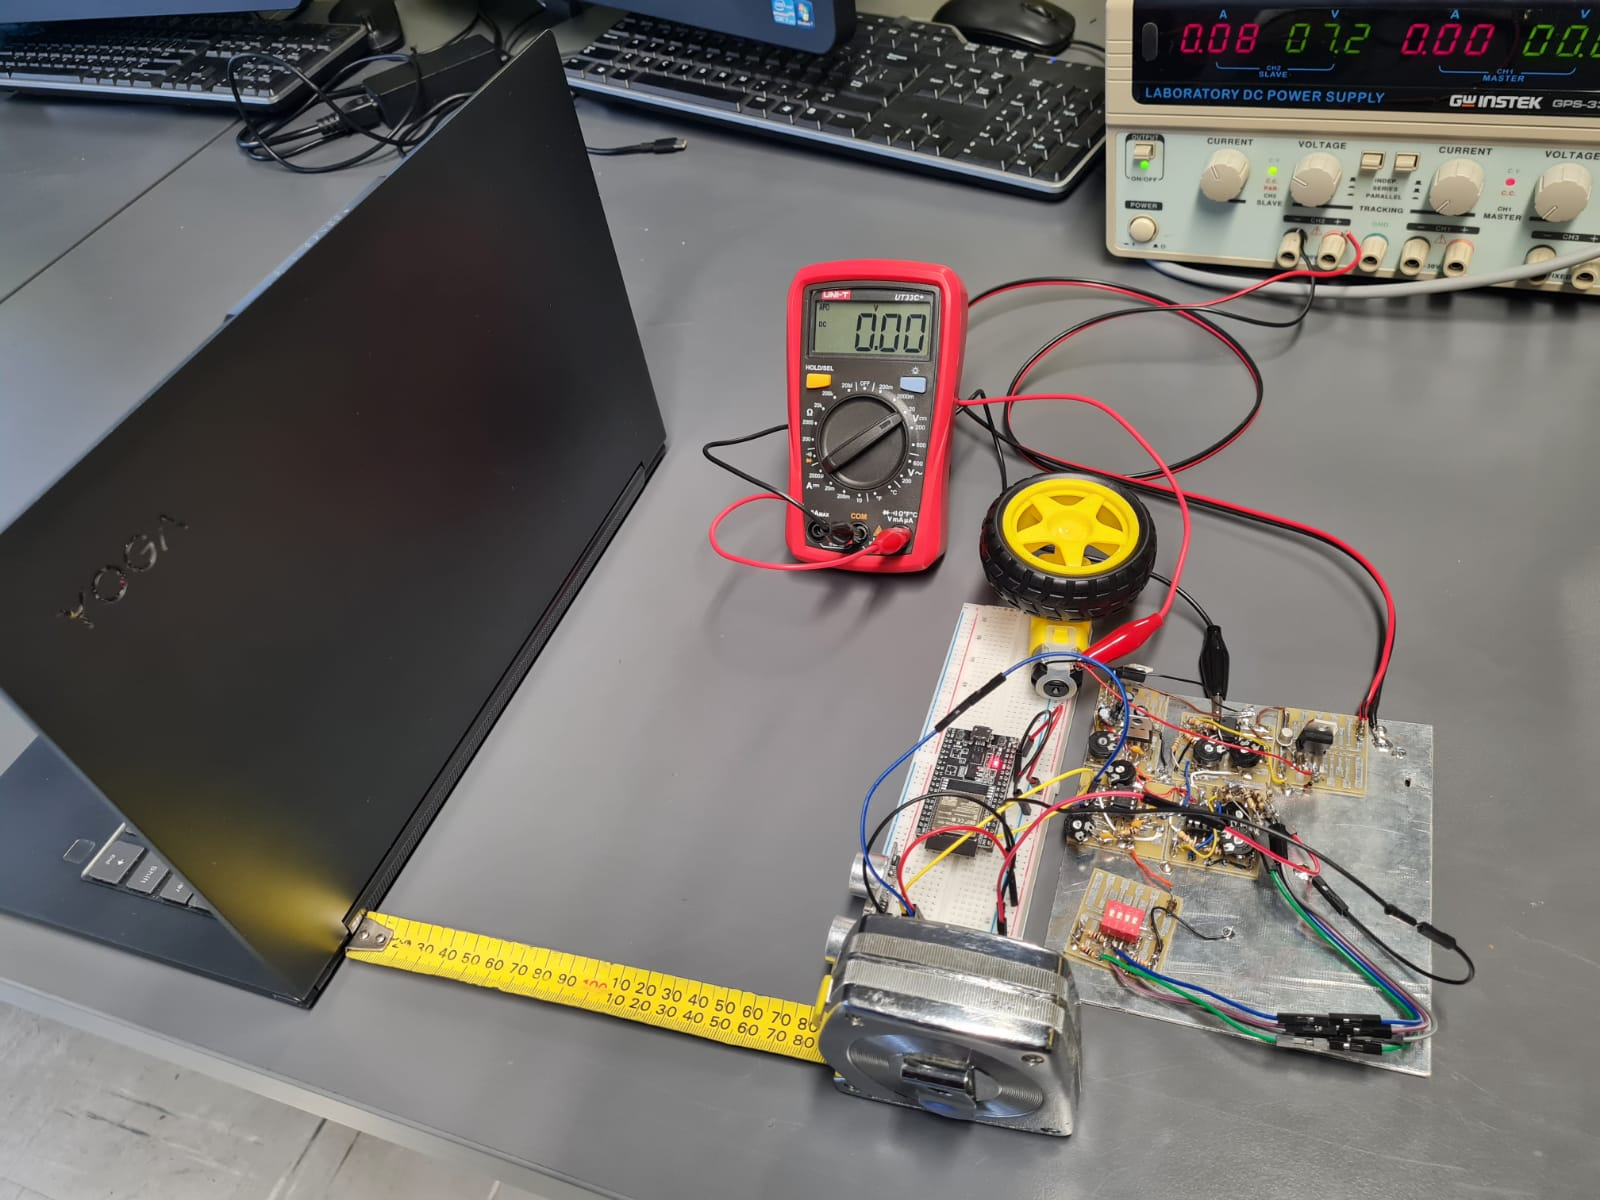
\includegraphics[width=1.0\linewidth]{motorController_near_0000}
        \captionof{figure}{Motor Voltage: Object Near, Speed 0000}
        \label{fig:motorController_near_0000}
    \end{minipage}
    \begin{minipage}{.38\textwidth}
        \centering
        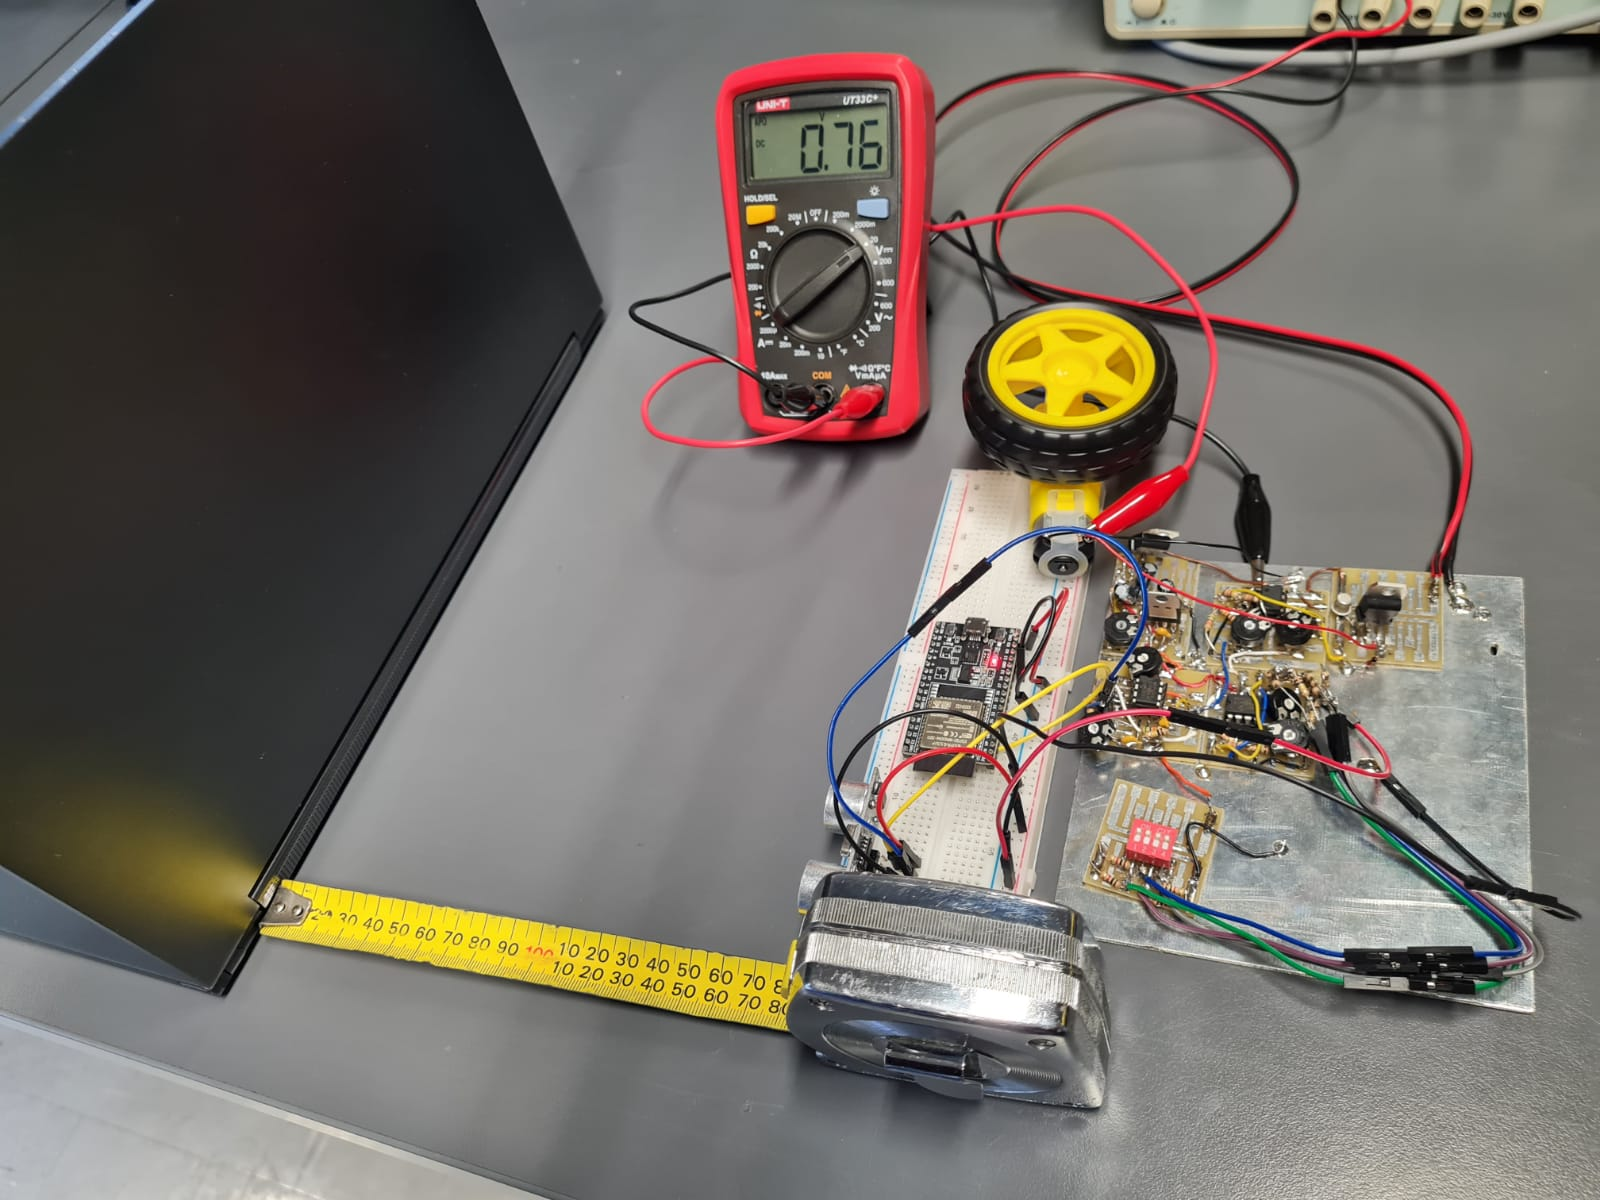
\includegraphics[width=1.0\linewidth]{motorController_near_1111}
        \captionof{figure}{Motor Voltage: Object Near, Speed 1111}
        \label{fig:motorController_near_1111}
    \end{minipage}
\end{figure}

The above four conditions show that the requirements were adhered to, in that the voltage is high $> \SI{5.5}{V}$
when the object is far and the torque command is a maximum, and the voltage is low $< \SI{0.5}{V}$ in all other edge-cases.

The designed $\SI{20}{cm}$ threshold was also measured, with the voltage resultant being $\SI{0.76}{V}$ as shown in Figure \ref{fig:motorController_20cm_1111}.
Although this was designed to equal 0.6 V at 20 cm, the motor is switched off at 0.76 V, and so the final requirement was still met.

\begin{figure}[!htb]
  \centering
  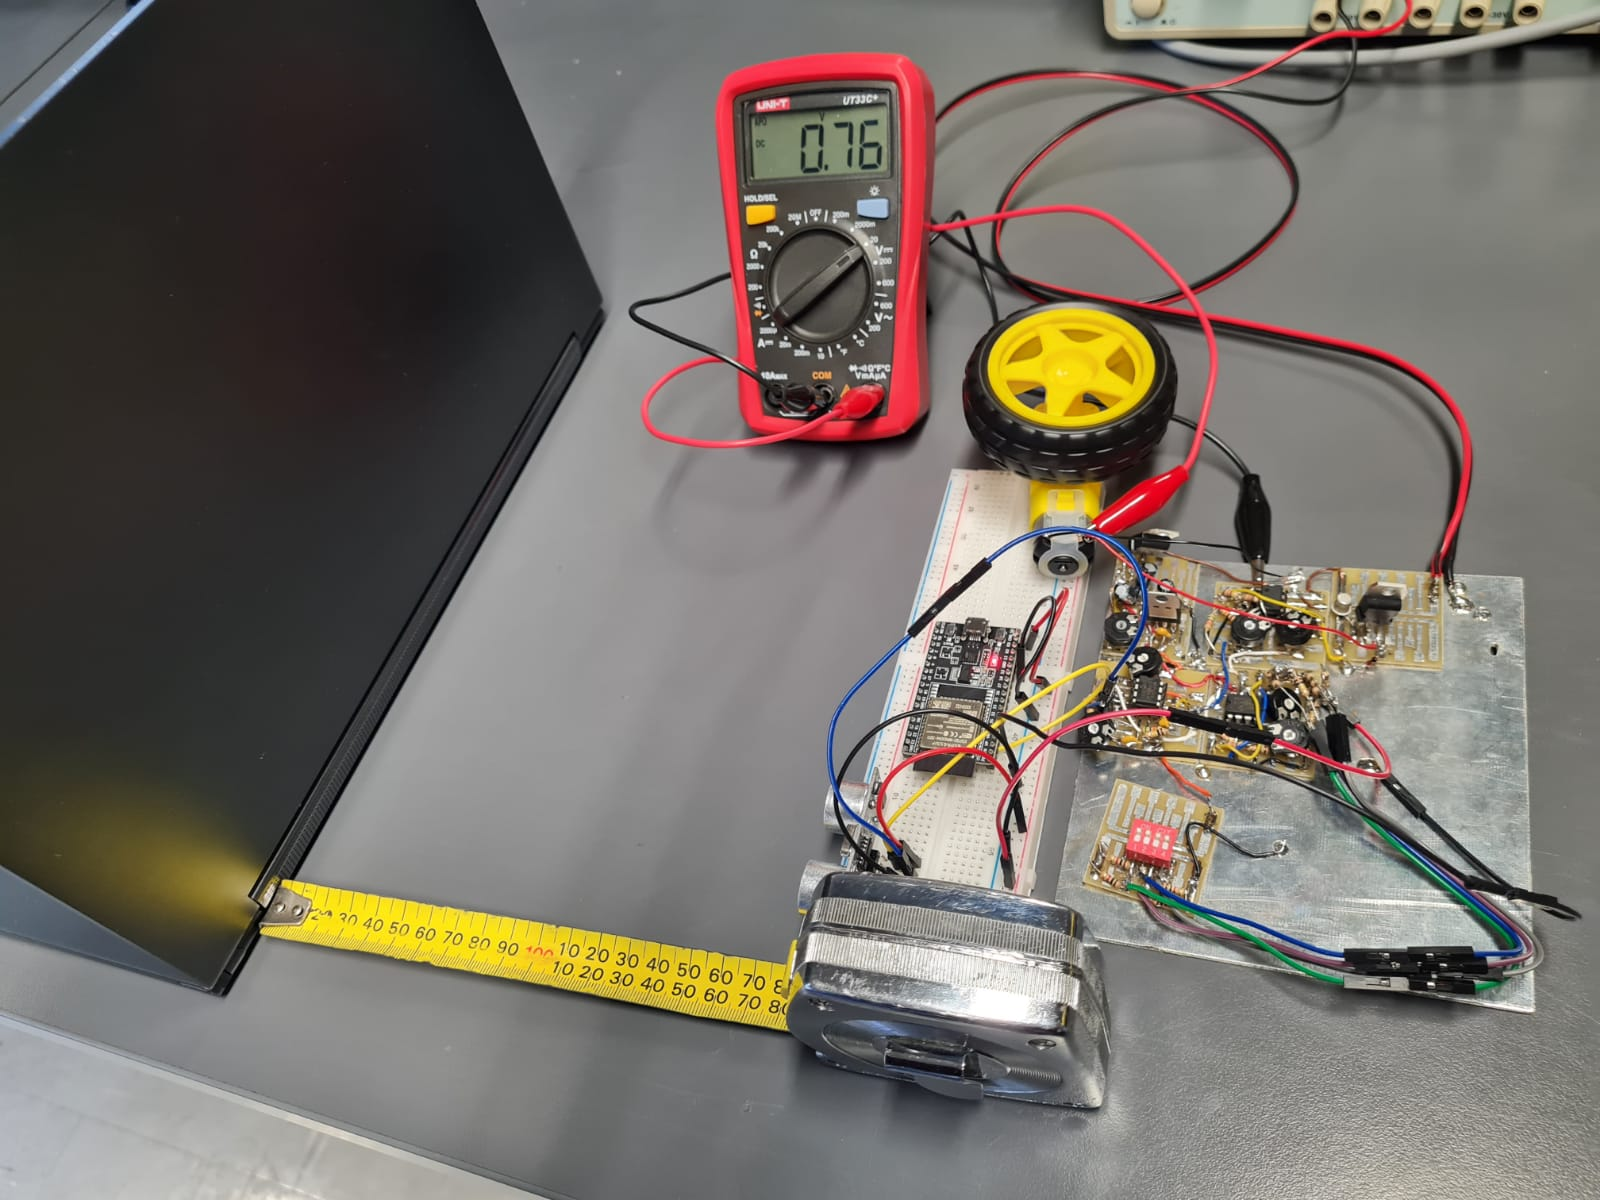
\includegraphics[width=0.3\textwidth]{motorController_20cm_1111}
  \caption{Motor Voltage: Object 20cm, Speed 1111}
  \label{fig:motorController_20cm_1111}
\end{figure}
\graphicspath{{content/2_design/figures/}}
\section{Digital Motor Controller: Firmware}

\subsection{Flow Diagrams}

\begin{figure}[!htb]
    \centering
    \begin{minipage}{.45\textwidth}
        \centering
        \fbox{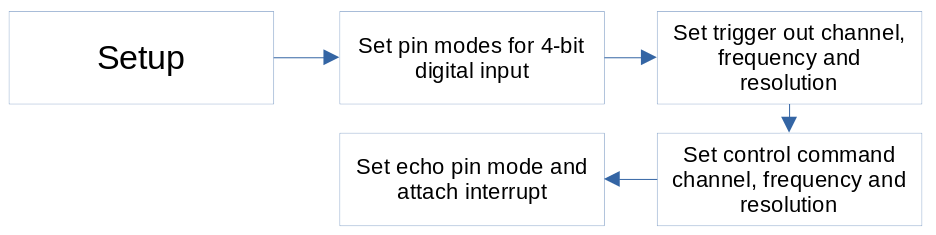
\includegraphics[width=0.9\linewidth]{digitalMotorController_flowChart_setup}}
        \captionof{figure}{Setup Diagram}
        \label{fig:digitalMotorController_flowChart_setup}
    \end{minipage}
    \begin{minipage}{.45\textwidth}
        \centering
        \fbox{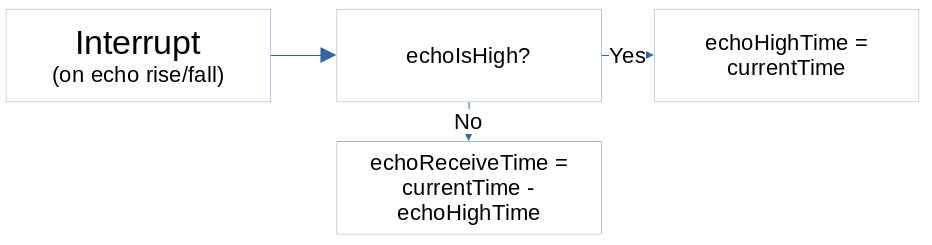
\includegraphics[width=0.9\linewidth]{digitalMotorController_flowChart_interrupt}}
        \captionof{figure}{Echo Interrupt Diagram}
        \label{fig:digitalMotorController_flowChart_interrupt}
    \end{minipage}
    \begin{minipage}{.45\textwidth}
        \centering
        \fbox{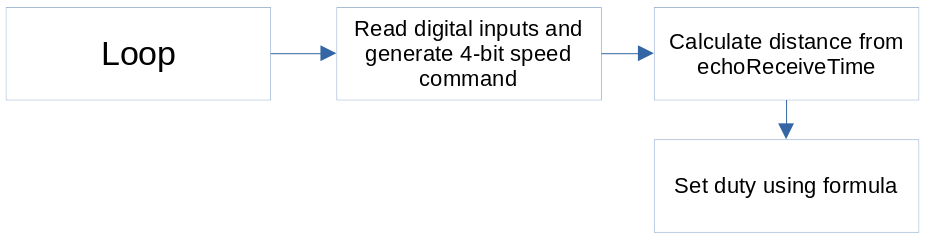
\includegraphics[width=0.9\linewidth]{digitalMotorController_flowChart_loop}}
        \captionof{figure}{Loop Diagram}
        \label{fig:digitalMotorController_flowChart_loop}
    \end{minipage}
\end{figure}

\subsection{Range Measurement}

As visible in Figure \ref{fig:digitalMotorController_flowChart_interrupt}, range will be calculated by measuring the time that the echo pin is high. An interrupt will be used to detect when
the echo output changes from low to high, and vice versa. Then, this time will be divided by two and multiplied by the speed of sound to determine
the range of the object. Since the time distance will be in microseconds, the following formula may be used: $D = \frac{t_{us}}{2} \times \SI{343}{m \cdot s^{-1}} \times 10^{-6}$.

\subsection{PWM Control}

\subsubsection{Frequency}

If $f_{PWM}$ is too low, the motor switching will be noticeable. If it is too high, the MOSFET will not turn on fast enough.
The motor's resistance was measured as $R = \SI{5.3}{\ohm}$, and inductance was calculated as $L = \SI{1.6}{\milli\henry}$ using a frequency test.
The motor's cutoff frequency is therefore $f_c = \frac{R}{2 \pi L} = \frac{5.3}{2 \pi \times 1.6 \times 10^{-3}} \approx \SI{500}{Hz}$.
Since the FQD13N06L has a rise time of $t_{r(max)} = \SI{190}{ns}$, signals will only be affected at frequencies near $f_r = \frac{1}{\SI{190}{ns}} \approx \SI{5}{GHz}$.
$f_{PWM} = \SI{10}{kHz}$ could safely be chosen to ensure adequate filtering of wave harmonics, while not affecting switching times,
however $f_{PWM} = \SI{20}{kHz}$ is used to keep the switching frequency above human hearing.

\subsubsection{Formula}

The digital formula used should emulate the analog motor controller as closely as possible. The controller's range will therefore also be from 20 cm to 1 m
and will saturate at "digital rails". Given $S$, the 4-bit speed command, and $R$, the range, the following formulae may be used:
$C = \bar{R} - (1 - \bar{S})$ with $\bar{R} = \frac{R - R_{min}}{R_{max} - R_{min}}$ and $\bar{S} = \frac{S}{15}$.
Finally $duty = clamp(0, C, 1) \times controlResolution$. LEDC functions can then be used \cite{ledControl} to set this PWM appropriately.
\graphicspath{{content/2_design/figures/}}
\section{Digital Motor Controller: Switch and Current Sensor}

\subsection{Configuration}

The low-side switch will be a FQD13N06L NMOS transistor driven by the ESP using PWM. This transistor was chosen due to its
low turn-on voltage, eliminating the need for any gain circuitry. A resistor will be used in series from the ESP to the MOSFET to
prevent surge currents due to the capacitive nature of the MOSFET gate. A pull-down resistor will also be used to ensure
the circuit is fully off when the ESP pin is in a high impedance state (e.g. when the circuit is powered down or during startup).

The current sensor circuit will also be a non-inverting amplifier with a filter, similar to the circuit used for the analog wheel,
however care needs to be taken to ensure the PWM signal is filtered adequately. The sense resistor will be placed on the low side
of the MOSFET to avoid the use of a differential amplifier.

\subsection{Input Resistors}

In order to calculate $R_a$, the series input resistor from the ESP, the assumption is made that the series resistance before the equivalent gate capacitance is zero.
Since the current equation for an RC circuit is $I(t) = I_0 e^{-t/\tau}$, with $I_0 = \frac{V}{R}$, the surge current will be $I_0$ at $t = 0$. Choose $I_0 = \SI{10}{mA}$
$\therefore R_a = \frac{V_{cc}}{I_0} = \frac{\SI{3.3}{V}}{\SI{10}{mA}} = \SI{330}{\ohm}$.

The pull-down resistor should be chosen so that the ESP is not loaded during operation, thereby affecting the voltage. If it is chosen that this resistor consumes
maximum additional current of $\SI{100}{\micro\ampere}$, the resistor should then be $R_{b(min)} = \frac{\SI{3.3}{V}}{\SI{100}{\micro\ampere}} = \SI{33}{\kilo\ohm}$.
Choose $R_b = \SI{100}{\kilo\ohm}$.

\subsection{Transistor Requirements}

It should be checked that the FQD13N06L transistor is suitable with regards to turn-on voltage, current capabilities, and series resistance.
\begin{itemize}
    \item The $V_{gs}$ threshold voltage should be checked to ensure the transistor is turned on fully. According to \cite{datasheetFQD13N06L},
          the maximum turn-on voltage of the transistor is 2.5 V. Since the ESP will output a 3.3 V PWM signal on its digital pins,
          the transistor will be turned on fully since the pin's output voltage is 32\% higher than the required $V_{gs}$ threshold.
    \item The current requirements should be compared with the transistor's current capabilities. A maximum stall current of 750 mA is required.
          If the transistor is not capable of handling this, it might be damaged due to excess heat dissipation. Choose $I_{max} = \SI{1}{A}$ for additional headroom.
          Again, according to \cite{datasheetFQD13N06L}, the transistor can handle a continuous current of $\SI{7}{A}$ with its case kept at \SI{100}{\celsius}. This is well
          within the current limitation of the motor.
    \item The equivalent series resistance of the transistor should be analyzed at different forward currents in order to determine the voltage drop it will cause
          in series with the motor. The datasheet reveals that, at $V_{gs} = \SI{5}{V}$, the forward resistance only varies from around $\SI{110}{\milli\ohm}$ to $\SI{120}{\milli\ohm}$
          as current increases to 10 A. At currents of around 1 A, a maximum voltage drop of around 0.12 V will be found, which is negligible and means that the motor will receive almost the
          full 7.2 V. This is also at maximum current - at lower current levels, the voltage drop will be even less, however in this design this will be slightly countered by the fact that
          $V_{gs} = \SI{3.3}{V}$.
\end{itemize}

\subsection{Current Sensor}

The same design as in \ref{design_currentSensor} will be used. Since a PWM frequency of 20 kHz will be used, the current sensor filtering frequency,
which is designed to adequately filter out a 1 kHz signal, is more than adequate, and will filter out the fundamental frequency and all harmonics.
The frequency could even be raised, however will be kept the same in order to match it with the analog wheel current sensor.

The rest of the design of the sensor can also be kept identical due to the final receiver of the value (the ESP) being the same. These design decisions, as well as the justifications
to keep them, are documented below:
\begin{itemize}
    \item The non-inverting gain will be 825, which allows for current values of up to 400 mA to be read.
    \item The filter cutoff frequency will remain at 11 Hz to have a slower response which heavily filters out any noise.
    \item A 3.3 V supply will be used to limit the output and prevent damaging the ESP's input pins.
\end{itemize}

\subsection{Circuit Diagram}

\begin{figure}[!htb]
  \centering
  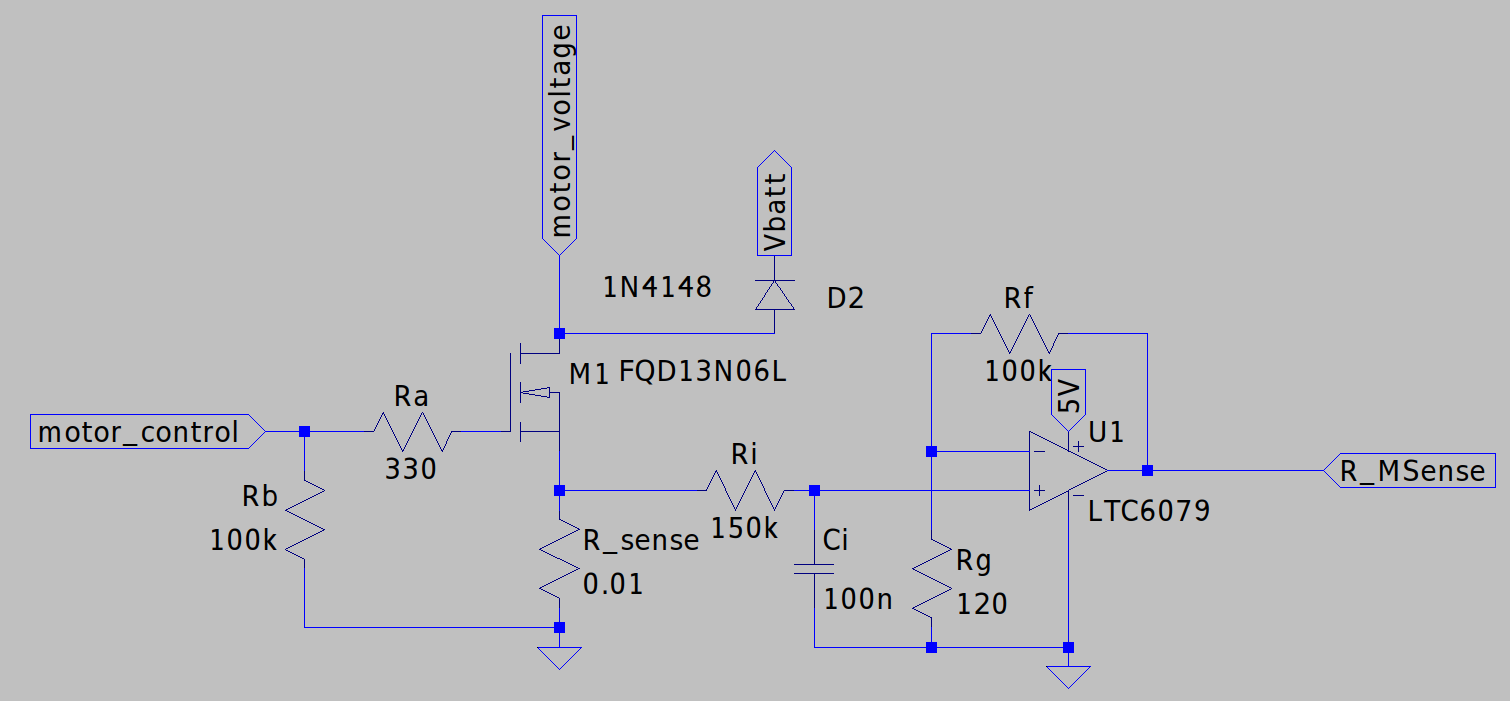
\includegraphics[width=0.7\textwidth]{digitalMotorController_circuitDiagram}
  \caption{Digital Motor Controller and Current Sensor Circuit Diagram}
  \label{fig:digitalMotorController_circuitDiagram}
\end{figure}
\chapter{Results}\label{ch:results}

\graphicspath{{content/4_implementation/figures/}}
\section{Current sensor}\label{sec:current_sensor_physical}

The implementation of the circuit was different in two ways compared to the original design:
\begin{itemize}
   \item \SI{120}{\kilo\ohm} resistors were used instead of \SI{100}{\kilo\ohm}, as they were easier to obtain, and would only result in a
         slightly larger gain and lower cutoff.
   \item The amplifier circuit was powered with regulated \SI{3.3}{V}. This was done to protect the ESP's input pins by saturating the output
         when it would have been too large.
\end{itemize}

\begin{figure}[!htb]
  \centering
  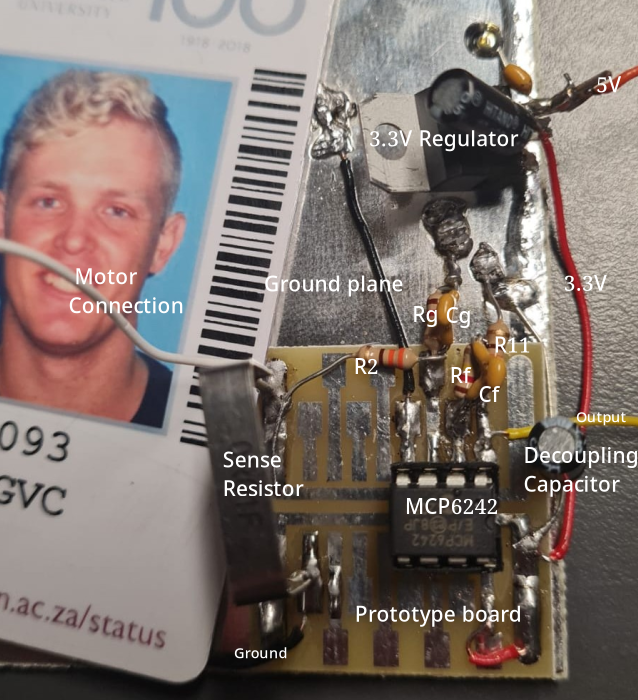
\includegraphics[width=0.75\textwidth]{currentSensor_impl_circuit}
  \caption{Final Circuit Implementation}
\end{figure}
\graphicspath{{content/2_design/figures/}}
\section{Range sensor}
\subsection{Sensor power \& output}{\label{rangeSensor_powerOutput}}
The range sensor requires \SI{5}{V_{dc}} power and will draw around \SI{15}{mA}. Since the LD1117V provides a stable 5.0 V output and is capable
of providing up to 800 mA of current, the sensor will be powered directly from this regulator.

The sensor's echo output is a PWM wave of varying duty cycle $\tau$ and $f_{PWM} = \SI{16}{Hz}$.
This signal's amplitude could be as high as 5 V (TTL level). The maximum output $A_{max}$ \textit{after} unity filtering,
however, will be determined by the maximum duty cycle, $t_{max}$. Since a distance of $D_{max} = \SI{1}{m}$ and $D_{min} = \SI{5}{cm}$,
Equations \ref{eqn:sensor_distanceFormula} and \ref{eqn:pwm_filtered_amplitude} can be used to calculate:
\begin{itemize}
  \item At $D_{max}$, $t_{max} \approx \SI{5.9}{ms}$, $\tau_{max} = \frac{\SI{5.9}{ms}}{1/16} \approx 9.5 \%$ and $A_{max} = (\SI{5}{V}) \cdot (9.5 \%) = \SI{475}{mV} $.
  \item At $D_{min}$, $t_{min} \approx \SI{0.29}{ms}$, $\tau_{min} = \frac{\SI{0.29}{ms}}{1/16} \approx 0.47 \%$ and $A_{min} = (\SI{5}{V}) \cdot (0.47 \%) = \SI{23}{mV} $.
\end{itemize}

\subsection{Filter selection}{\label{rangeSensor_filterSelection}}

To determine the filter's order, rise time and noise requirements should be considered:
\begin{itemize}
  \item After filtering, since gain $\approx \frac{\SI{3}{V}}{\SI{475}{mV}} \approx \SI{7}{V/V}$, filter ripple must be under $ \frac{\SI{70}{mV}}{7} = \SI{7}{mV}$.
  \item A 10\% to 90\% rise time ($t_r$) of \SI{1.5}{s} should be adhered to.
\end{itemize}

\noindent These specifications result in the requirement that $A_{dB}$ at $f_{PWM} = 20 \log \left[ \frac{\SI{5}{V}}{\SI{7}{mV}} \right] \approx \SI{60}{dB}$.
A \nth{3} order filter with $f_c = \SI{1}{Hz}$ will be used, as a \nth{2} order may be tolerance-sensitive.
This provides $t_r \approx 0.63 s$ and $A_{dB} \approx 72 dB $ [\ref{filter_formulae}].

\begin{table}[!h]
  \centering
  \renewcommand{\arraystretch}{1.2}
  \begin{tabular}{ |c|c|p{2.5cm}|p{2.5cm}|p{3.5cm}| }
    \hline
    \textbf{Filter type}  & \textbf{Design Spec.}         & \textbf{Cutoff $f_c$}     & \textbf{Rise time $t_r$}        & \textbf{Attenuation $A_{dB}$}       \\
    \hline
    \nth{1} order            & Rise Time                     & 0.233 Hz                  & 1.5 s                           & 37 dB                               \\
                             & Attenuation                   & 0.016 Hz                  & 22 s                            & 60 dB                               \\ \hline
    \nth{2} order            & Rise Time                     & 0.350 Hz                  & 1.5 s                           & 66 dB                               \\
                             & Attenuation                   & 0.505 Hz                  & 1.038 s                         & 60 dB                               \\ \hline
    \nth{3} order (cascade)  & Rise Time                     & 0.420 Hz                  & 1.5 s                           & 95 dB                               \\
                             & Attenuation                   & 1.600 Hz                  & 0.394 s                         & 60 dB                               \\ \hline
  \end{tabular}
  \caption{Filter type vs Rise Time and Attenuation using [\ref{filter_formulae}]}
  \label{tab:range_sensor_filter_comparison}
\end{table}

\subsection{Configuration}\label{rangeSensor_circuitConfig}

A "two-and-a-half" stage configuration will be used. The first stage is a gain/offset and \nth{1} order filter,
and is placed first in order to amplify the signal above the MCP's 35 mV floor. The second stage is unity-gain \nth{2} order filter.
A non-inverting amplifier will be used for stage 1, and a Sallen-Key topology for stage 2. Since the quiescent current for each op-amp is
$\SI{70}{uA}$ \cite{datasheetMCP6242}, stage 1 \& 2 will be allocated $\SI{400}{\micro\ampere}$ and $\SI{200}{\micro\ampere}$ respectively.

\begin{figure}[!htb]
  \centering
  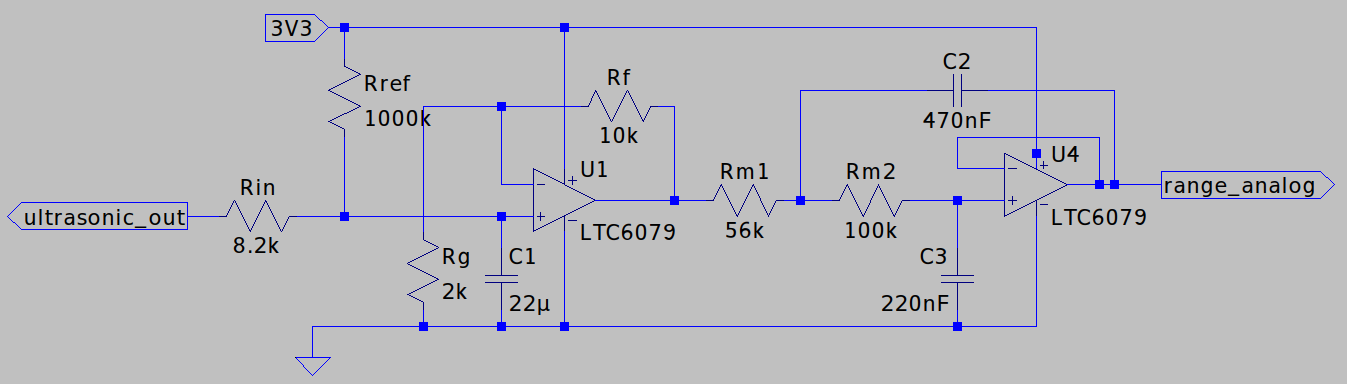
\includegraphics[width=0.8\textwidth]{rangeSensor_circuitDiagram}
  \caption{Final range sensor amplifier circuit diagram}
  \label{fig:rangeSensor_circuitDiagram}
\end{figure}

\subsection{Gain stage}

This stage will be powered by the 3.3 V regulator. As this is a low-gain circuit, input bias voltages can be neglected.
Slew rate and CMMR imbalance can also be ignored due to the low-frequency, single-ended use of the op-amp.
Voltage rail saturation does not need to be considered at the circuit output, as $\SI{0.3}{V} < V_{out} < \SI{3}{V}$,
and has already been catered for at the input, as discussed in Section \ref{rangeSensor_circuitConfig}.
Using the equations at \cite{gainOffset30Seconds}, and the expected input ranges from the filter stage,
gain $m = \frac{\SI{3}{V} - \SI{0.3}{V}}{\SI{475}{mV} - \SI{23}{mV}} = \SI{5.97}{\volt\per\volt}$,
and offset $b = \SI{0.3}{V} - m \times \SI{23}{mV} \approx \SI{163}{mV}$:

\begin{itemize}
  \item With idle current $I_Q = \frac{V_{out}}{R_f + R_g}$, and $V_{out(max)} = \SI{3.3}{V}$, $(R_f + R_g)_{min} = \frac{\SI{3.3}{V}}{\SI{400}{\micro\ampere}} = \SI{8.25}{\kilo\ohm}$.
  \item Since the offset voltage is low (i.e. $R_{ref}$ will be high), first choose $R_{ref} = \SI{820}{\kilo\ohm} + \SI{470}{\kilo\ohm} \textnormal{pot} \approx \SI{1000}{\kilo\ohm}$.
        A potentiometer is used to tune the offset.
  \item Calculate $R_{in} = \frac{R_{ref} \times b}{V_{ref} \times m} \approx \SI{8.2}{\kilo\ohm}$ with $V_{ref} = \SI{5}{V}$ and $C_1 = \frac{1}{2 \pi f_c R_1} \approx \SI{22}{\micro\farad}$.
  \item Choose $R_f = \SI{10}{\kilo\ohm}$ to satisfy the current requirements.
  \item Calculate $R_g = \frac{R_{ref} \times R_f}{m \times (R_{in} + R_{ref}) - R_{ref}} \approx \SI{2}{\kilo\ohm}$. To tune the gain, choose $R_g = \SI{1.5}{k} + \SI{1}{\kilo\ohm}\textnormal{pot}$.
\end{itemize}


\subsection{Filter stage}{\label{rangeSensor_filterDesign}}

This stage will use the 3.3 V regulator to clip the circuit output for use with the MCU.
This results in the \nth{2} order stage transfer function $H(s) = \frac{1}{1 + 0.2251 s + 0.02533 s^2} = \frac{1}{1 + a_1 s + b_1 s^2}$ with $\zeta = 0.707$. Now, component values can be chosen.
Formulae from \cite{filterDesign} will be used:

\begin{itemize}
  \item Since both capacitors are open-circuit during DC, the idle current is very low. A maximum step input will result in a surge of current through $C_2$ to ground.
        With $V_{in(max)} = \SI{5}{V}$, $(R_{m1} + R_{m2})_{min} = \frac{\SI{5}{V}}{\SI{200}{\micro\ampere}} = \SI{25}{\kilo\ohm}$.
  \item Since $C_3 = \frac{a_1}{2 \pi f_c (R_{m1} + R_{m2})}$ \cite{filterDesign}, choose $C_3 = \SI{220}{nF}$ so that $R_{m1} + R_{m2} \approx \SI{160}{\kilo\ohm}$.
  \item To meet $C_2 \geq C_3 \cdot \frac{4 \cdot b_1}{a_1 ^2} \approx 2 C_3 $ \cite{filterDesign}, choose $C_2 = \SI{470}{nF}$.
  \item Since $C_3 \cdot C_2 = \frac{b_1}{((2 \pi f_c)^2 R_{m1} R_{m2})}$, and $R_{m1} + R_{m2} = \SI{450}{\kilo\ohm}$, solve to obtain $R_{m1} = \SI{61}{\kilo\ohm}$ and $R_{m2} = \SI{99}{\kilo\ohm}$.
        Choose $R_{m1} = \SI{56}{\kilo\ohm}$ and $R_{m2} = \SI{100}{\kilo\ohm}$ as practical values.
\end{itemize}
\chapter{Physical Implementation}\label{ch:implementation}

\graphicspath{{content/4_implementation/figures/}}
\section{Current sensor}\label{sec:current_sensor_physical}

The implementation of the circuit was different in two ways compared to the original design:
\begin{itemize}
   \item \SI{120}{\kilo\ohm} resistors were used instead of \SI{100}{\kilo\ohm}, as they were easier to obtain, and would only result in a
         slightly larger gain and lower cutoff.
   \item The amplifier circuit was powered with regulated \SI{3.3}{V}. This was done to protect the ESP's input pins by saturating the output
         when it would have been too large.
\end{itemize}

\begin{figure}[!htb]
  \centering
  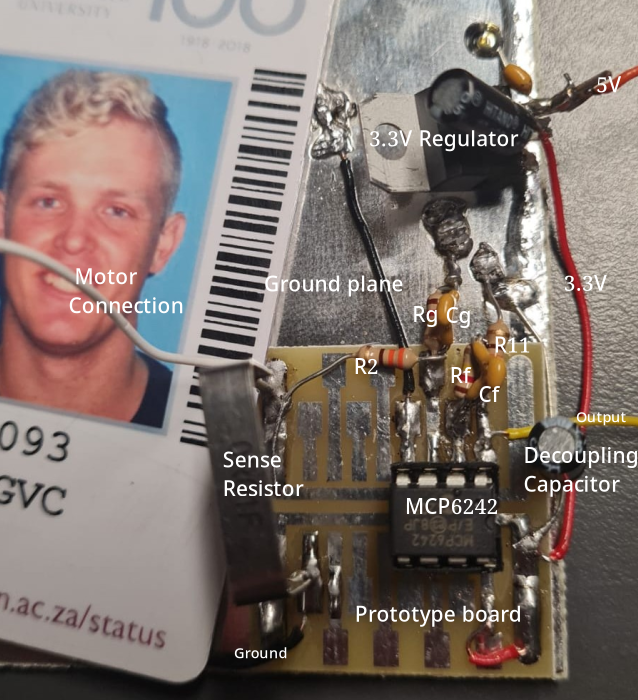
\includegraphics[width=0.75\textwidth]{currentSensor_impl_circuit}
  \caption{Final Circuit Implementation}
\end{figure}
\pagebreak
\graphicspath{{content/2_design/figures/}}
\section{Ultrasonic Sensor}
\subsection{Power and Output Requirements}
The range sensor requires \SI{5}{V_{dc}} power and will draw around \SI{15}{mA}. Since the LD1117V provides a stable 5.0 V output and is capable
of providing up to 800 mA of current, the sensor will be powered directly from this regulator.

The sensor's echo output is a PWM wave of varying duty cycle $\tau$ and $f_{PWM} = \SI{16}{Hz}$.
This signal's amplitude could be as high as 5 V (TTL level). The maximum output $A_{max}$ \textit{after} unity filtering,
however, will be determined by the maximum duty cycle, $t_{max}$. Since a distance of $D_{max} = \SI{1}{m}$ and $D_{min} = \SI{5}{cm}$,
Equations \ref{eqn:sensor_distanceFormula} and \ref{eqn:pwm_filtered_amplitude} can be used to calculate:
\begin{itemize}
  \item At $D_{max}$, $t_{max} \approx \SI{5.9}{ms}$, $\tau_{max} = \frac{\SI{5.9}{ms}}{1/16} \approx 9.5 \%$ and $A_{max} = (\SI{5}{V}) \cdot (9.5 \%) = \SI{475}{mV} $.
  \item At $D_{min}$, $t_{min} \approx \SI{0.29}{ms}$, $\tau_{min} = \frac{\SI{0.29}{ms}}{1/16} \approx 0.47 \%$ and $A_{min} = (\SI{5}{V}) \cdot (0.47 \%) = \SI{23}{mV} $.
\end{itemize}

\subsection{Filter Selection}{\label{rangeSensor_filterSelection}}

To determine the filter's order, rise time and noise requirements should be considered:
\begin{itemize}
  \item After filtering, since gain $\approx \frac{\SI{3}{V}}{\SI{475}{mV}} \approx \SI{7}{V/V}$, filter ripple must be under $ \frac{\SI{70}{mV}}{7} = \SI{7}{mV}$.
  \item A 10\% to 90\% rise time ($t_r$) of \SI{1.5}{s} should be adhered to.
\end{itemize}

\noindent These specifications result in the requirement that $A_{dB}$ at $f_{PWM} = 20 \log \left[ \frac{\SI{5}{V}}{\SI{7}{mV}} \right] \approx \SI{60}{dB}$.
A \nth{3} order filter with $f_c = \SI{1}{Hz}$ will be used, as a \nth{2} order may be tolerance-sensitive.
This provides $t_r \approx 0.63 s$ and $A_{dB} \approx 72 dB $ [\ref{filter_formulae}].

\begin{table}[!h]
  \centering
  \renewcommand{\arraystretch}{1.2}
  \begin{tabular}{ |c|c|p{2.5cm}|p{2.5cm}|p{3.5cm}| }
    \hline
    \textbf{Filter type}  & \textbf{Design Spec.}         & \textbf{Cutoff $f_c$}     & \textbf{Rise time $t_r$}        & \textbf{Attenuation $A_{dB}$}       \\
    \hline
    \nth{1} order            & Rise Time                     & 0.233 Hz                  & 1.5 s                           & 37 dB                               \\
                             & Attenuation                   & 0.016 Hz                  & 22 s                            & 60 dB                               \\ \hline
    \nth{2} order            & Rise Time                     & 0.350 Hz                  & 1.5 s                           & 66 dB                               \\
                             & Attenuation                   & 0.505 Hz                  & 1.038 s                         & 60 dB                               \\ \hline
    \nth{3} order (cascade)  & Rise Time                     & 0.420 Hz                  & 1.5 s                           & 95 dB                               \\
                             & Attenuation                   & 1.600 Hz                  & 0.394 s                         & 60 dB                               \\ \hline
  \end{tabular}
  \caption{Filter type vs Rise Time and Attenuation using [\ref{filter_formulae}]}
  \label{tab:range_sensor_filter_comparison}
\end{table}

\subsection{Configuration}{\label{rangeSensor_circuitConfig}}

A "two-and-a-half" stage configuration will be used. The first stage is a gain/offset and \nth{1} order filter,
and is placed first in order to amplify the signal above the MCP's 35 mV floor. The second stage is unity-gain \nth{2} order filter.
A non-inverting amplifier will be used for stage 1, and a Sallen-Key topology for stage 2. Since the quiescent current for each op-amp is
$\SI{70}{uA}$ \cite{datasheetMCP6242}, stage 1 \& 2 will be allocated $\SI{400}{\micro\ampere}$ and $\SI{200}{\micro\ampere}$ respectively.

\begin{figure}[!htb]
  \centering
  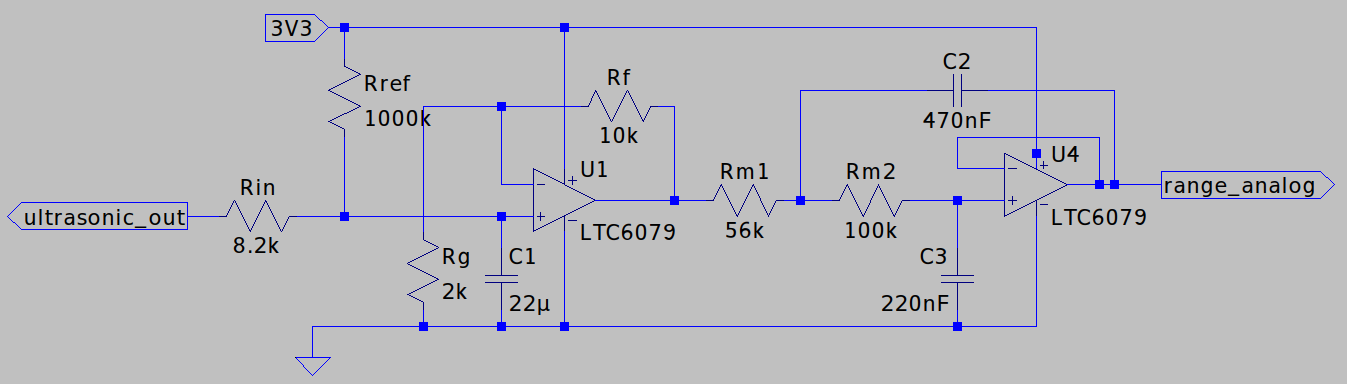
\includegraphics[width=0.8\textwidth]{rangeSensor_circuitDiagram}
  \caption{Range Sensor Amplifier Circuit Diagram}
  \label{fig:rangeSensor_circuitDiagram}
\end{figure}

\subsection{Gain Stage}

This stage will be powered by the 3.3 V regulator. As this is a low-gain circuit, input bias voltages can be neglected.
Slew rate and CMMR imbalance can also be ignored due to the low-frequency, single-ended use of the op-amp.
Voltage rail saturation does not need to be considered at the circuit output, as $\SI{0.3}{V} < V_{out} < \SI{3}{V}$,
and has already been catered for at the input, as discussed in Section \ref{rangeSensor_circuitConfig}.
Using the equations at \cite{gainOffset30Seconds}, and the expected input ranges from the filter stage,
gain $m = \frac{\SI{3}{V} - \SI{0.3}{V}}{\SI{475}{mV} - \SI{23}{mV}} = \SI{5.97}{\volt\per\volt}$,
and offset $b = \SI{0.3}{V} - m \times \SI{23}{mV} \approx \SI{163}{mV}$:

\begin{itemize}
  \item With idle current $I_Q = \frac{V_{out}}{R_f + R_g}$, and $V_{out(max)} = \SI{3.3}{V}$, $(R_f + R_g)_{min} = \frac{\SI{3.3}{V}}{\SI{400}{\micro\ampere}} = \SI{8.25}{\kilo\ohm}$.
  \item Since the offset voltage is low, $R_{ref}$ will be high. A potentiometer will also be used to tune this offset, therefore choose $R_{ref} = \SI{1000}{\kilo\ohm} = \SI{820}{\kilo\ohm} + \SI{470}{\kilo\ohm} \textnormal{pot}$.
  \item Calculate $R_{in} = \frac{R_{ref} \times b}{V_{ref} \times m} \approx \SI{8.2}{\kilo\ohm}$ with $V_{ref} = \SI{5}{V}$ and $C_1 = \frac{1}{2 \pi f_c R_1} \approx \SI{22}{\micro\farad}$.
  \item Choose $R_f = \SI{10}{\kilo\ohm}$ to satisfy the current requirements.
  \item Calculate $R_g = \frac{R_{ref} \times R_f}{m \times (R_{in} + R_{ref}) - R_{ref}} \approx \SI{2}{\kilo\ohm}$. To tune the gain, choose $R_g = \SI{1.5}{k} + \SI{1}{\kilo\ohm}\textnormal{pot}$.
\end{itemize}


\subsection{Filter Stage}

This stage will use the 3.3 V regulator to clip the circuit output for use with the MCU.
This results in the \nth{2} order stage transfer function $H(s) = \frac{1}{1 + 0.2251 s + 0.02533 s^2} = \frac{1}{1 + a_1 s + b_1 s^2}$ with $\zeta = 0.707$. Now, component values can be chosen.
Formulae from \cite{filterDesign} will be used:

\begin{itemize}
  \item Since both capacitors are open-circuit during DC, the idle current is very low. A maximum step input will result in a surge of current through $C_2$ to ground.
        With $V_{in(max)} = \SI{5}{V}$, $(R_{m1} + R_{m2})_{min} = \frac{\SI{5}{V}}{\SI{200}{\micro\ampere}} = \SI{25}{\kilo\ohm}$.
  \item Since $C_3 = \frac{a_1}{2 \pi f_c (R_{m1} + R_{m2})}$ \cite{filterDesign}, choose $C_3 = \SI{220}{nF}$ so that $R_{m1} + R_{m2} \approx \SI{160}{\kilo\ohm}$.
  \item To meet $C_2 \geq C_3 \cdot \frac{4 \cdot b_1}{a_1 ^2} \approx 2 C_3 $ \cite{filterDesign}, choose $C_2 = \SI{470}{nF}$.
  \item Since $C_3 \cdot C_2 = \frac{b_1}{((2 \pi f_c)^2 R_{m1} R_{m2})}$, and $R_{m1} + R_{m2} = \SI{450}{\kilo\ohm}$, solve to obtain $R_{m1} = \SI{61}{\kilo\ohm}$ and $R_{m2} = \SI{99}{\kilo\ohm}$.
        Choose $R_{m1} = \SI{56}{\kilo\ohm}$ and $R_{m2} = \SI{100}{\kilo\ohm}$ as practical values.
\end{itemize}
\pagebreak
\graphicspath{{content/3_results/figures}}
\section{Digital to Analog Converter}

\subsection{Simulation}

\begin{figure}[!htb]
    \centering
    \begin{minipage}{.5\textwidth}
        \centering
        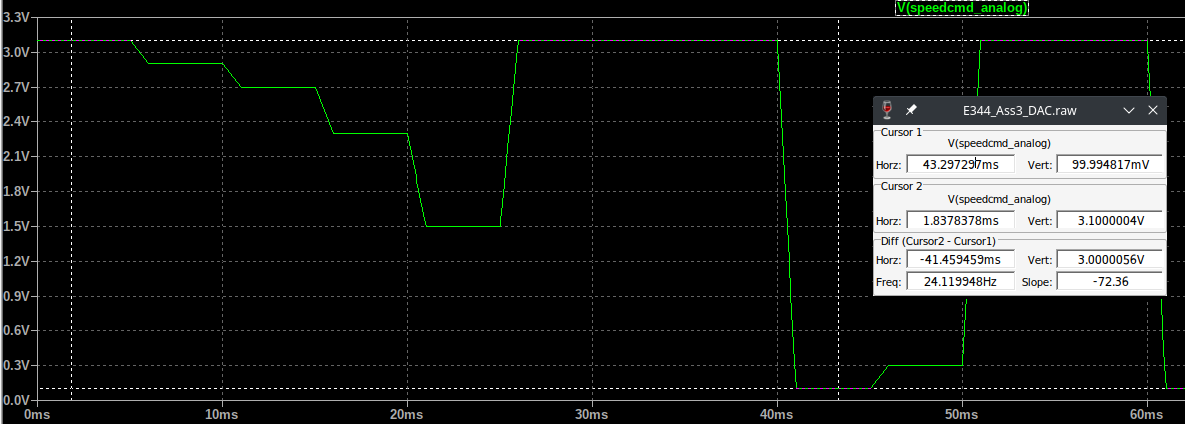
\includegraphics[width=1.0\linewidth]{dac_sim_range}
        \captionof{figure}{Output Range from 0000 (First Cursor) to 1111 (Second Cursor)}
        \label{fig:dac_sim_range}
    \end{minipage}
    \begin{minipage}{.45\textwidth}
        \centering
        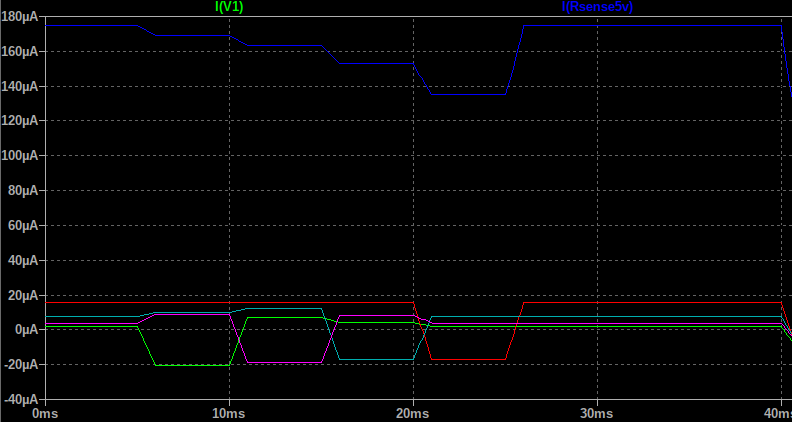
\includegraphics[width=1.0\linewidth]{dac_sim_currentDraw}
        \captionof{figure}{Current Draw (Amplifier and Digital Inputs)}
        \label{fig:dac_sim_currentDraw}
    \end{minipage}
\end{figure}

As seen in the above figures, all specifications were complied with:
\begin{itemize}
    \item Figure \ref{fig:dac_sim_range} shows that an output of 0000 produces exactly 3.1 V on the output, and that 1111 produces 100 mV.
    \item Figure \ref{fig:dac_sim_currentDraw} shows a maximum current draw of under $\SI{180}{\micro\ampere}$, which is much under the $\SI{250}{\micro\ampere}$ specification.
          It also shows that each digital input draws less than $\SI{20}{\micro\ampere}$, also under the $\SI{50}{\micro\ampere}$ specification.
\end{itemize}

\subsection{Implementation}

\begin{figure}[!htb]
    \centering
    \begin{minipage}{.22\textwidth}
        \centering
        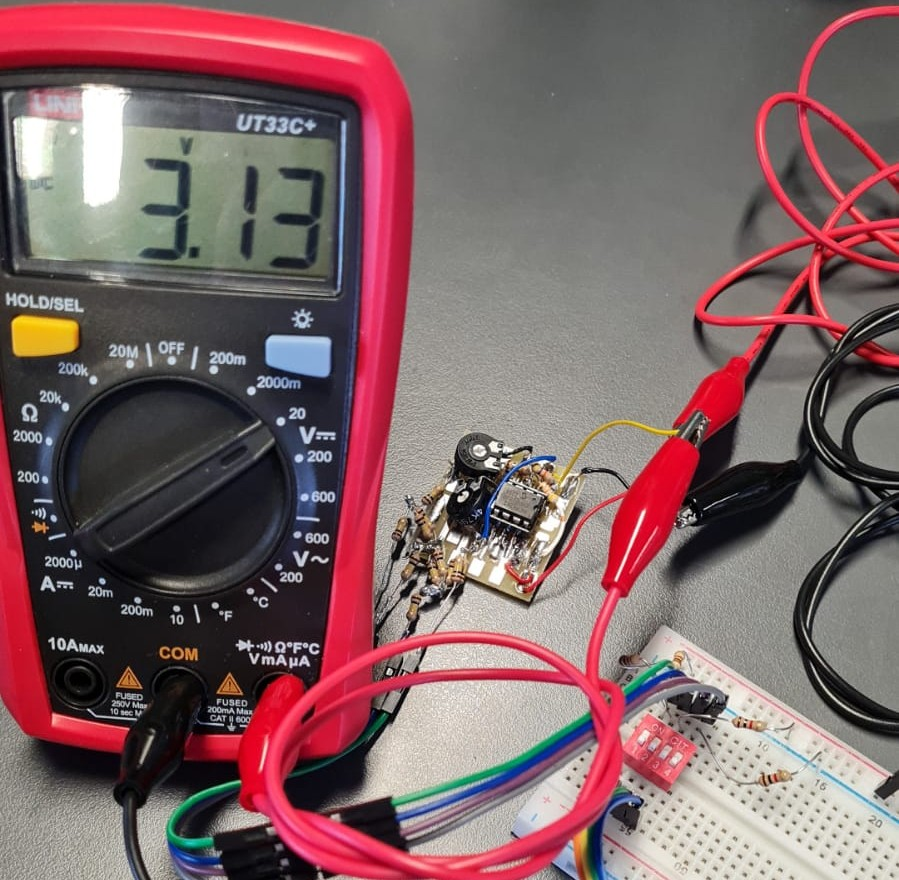
\includegraphics[width=1.0\linewidth]{dac_impl_0000}
        \captionof{figure}{DAC Output at 0000}
        \label{fig:dac_impl_0000}
    \end{minipage}
    \begin{minipage}{.2\textwidth}
        \centering
        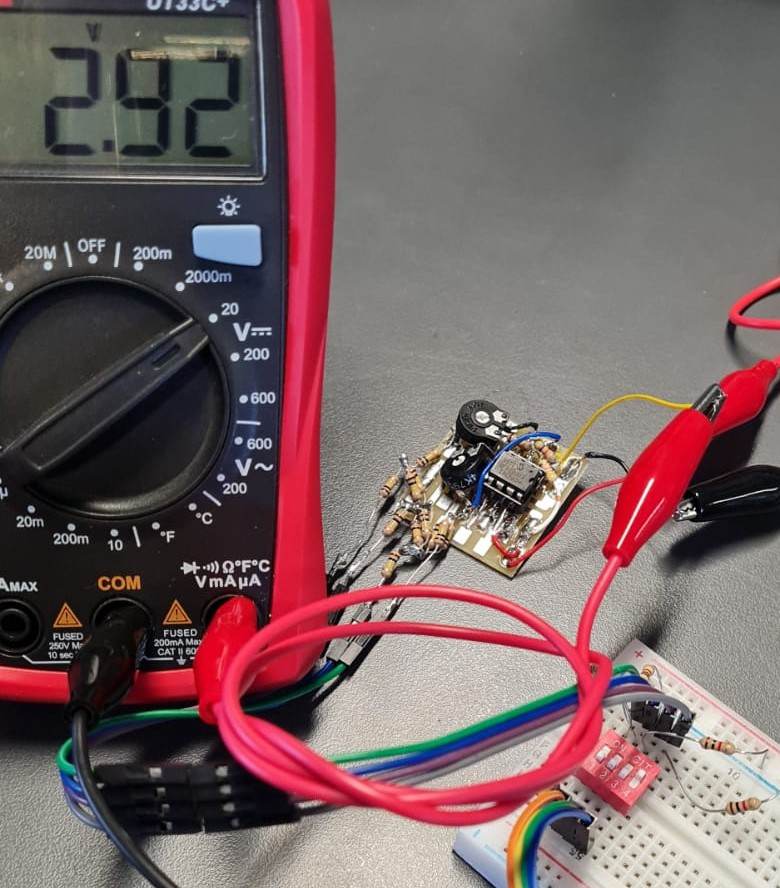
\includegraphics[width=1.0\linewidth]{dac_impl_0001}
        \captionof{figure}{DAC Output at 0001}
        \label{fig:dac_impl_0001}
    \end{minipage}
    \begin{minipage}{.22\textwidth}
        \centering
        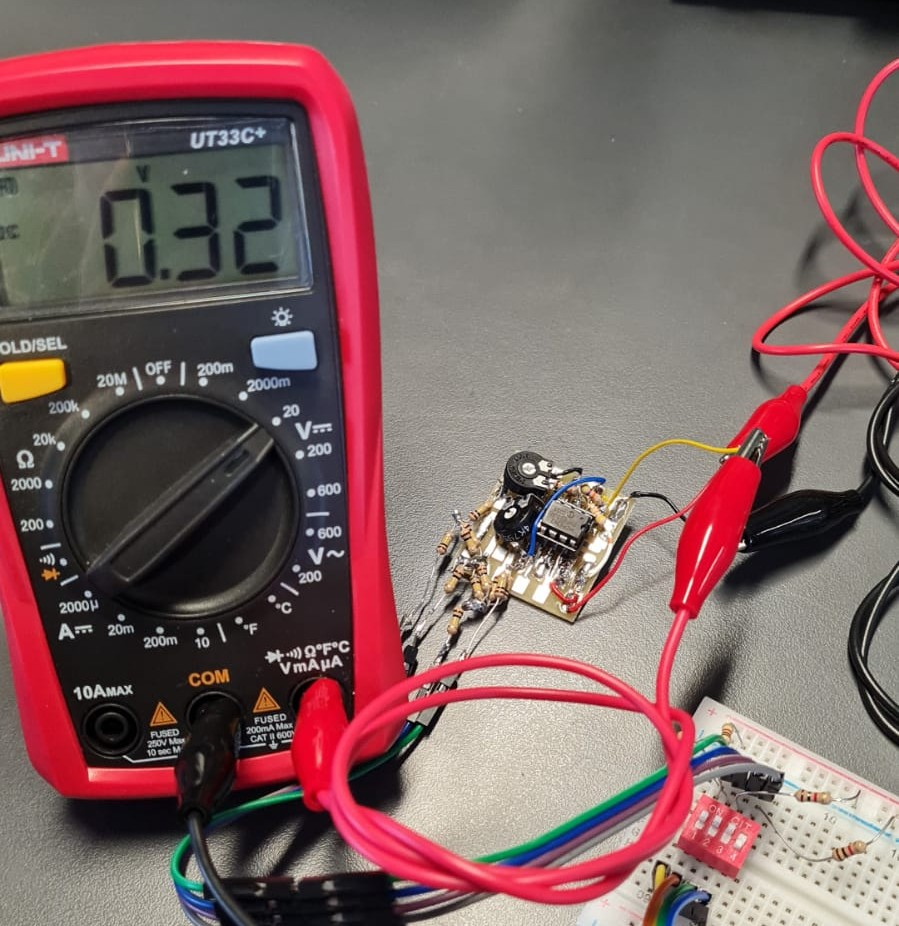
\includegraphics[width=1.0\linewidth]{dac_impl_1110}
        \captionof{figure}{DAC Output at 1110}
        \label{fig:dac_impl_1110}
    \end{minipage}
    \begin{minipage}{.2\textwidth}
        \centering
        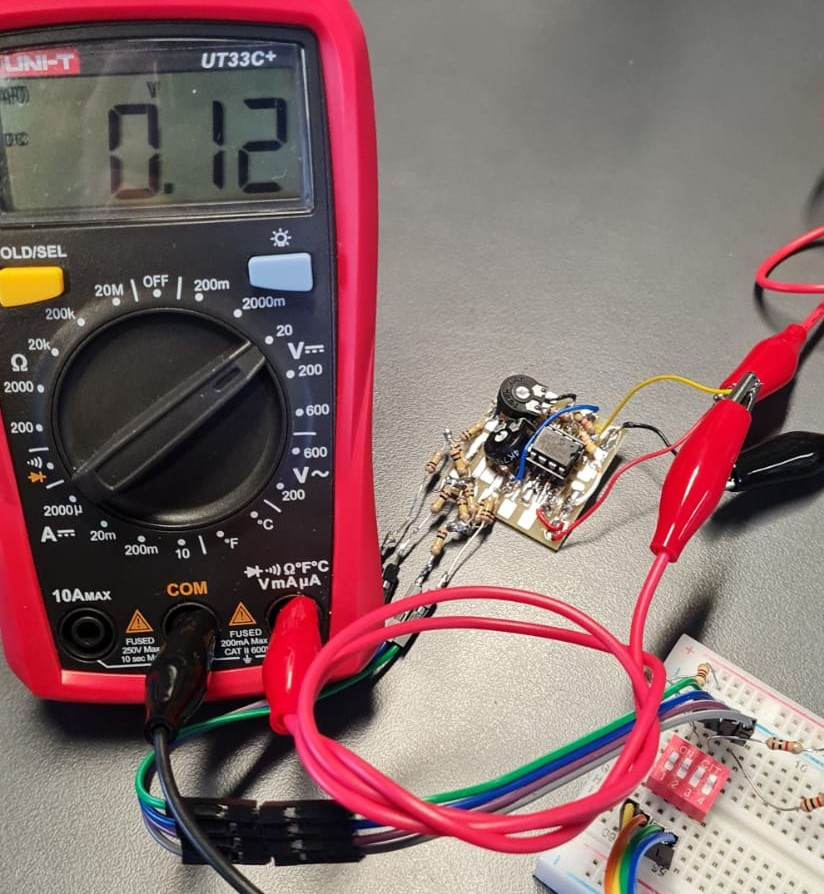
\includegraphics[width=1.0\linewidth]{dac_impl_1111}
        \captionof{figure}{DAC Output at 1111}
        \label{fig:dac_impl_1111}
    \end{minipage}    
\end{figure}

Figures \ref{fig:dac_impl_0000} to \ref{fig:dac_impl_1111} demonstrate the output voltages at specific digital input combinations.
All specifications are complied with, specifically that 0000 produces $> \SI{3}{V}$ on the output, and that 1111 produces $< \SI{0.5}{V}$.

% Bibliography
\bibliography{references}

% End matter
\appendix
\graphicspath{{endmatter/figures/}}
\chapter{Social contract}
\makeatletter\@mkboth{}{Appendix}\makeatother
\label{appen:social_contract}
     \begin{figure}[!htb]
     \centering
     	\fbox{
\includegraphics[width=0.8\linewidth]{SocialContract_signed.pdf}}
       \label{fig:social_contract}
	\end{figure}
\graphicspath{{endmatter/figures/}}
\chapter{GitHub Activity Heatmap}
\makeatletter\@mkboth{}{Appendix}\makeatother
\label{appen:github_heatmap}

     \begin{figure}[!htb]
     \centering
     	\fbox{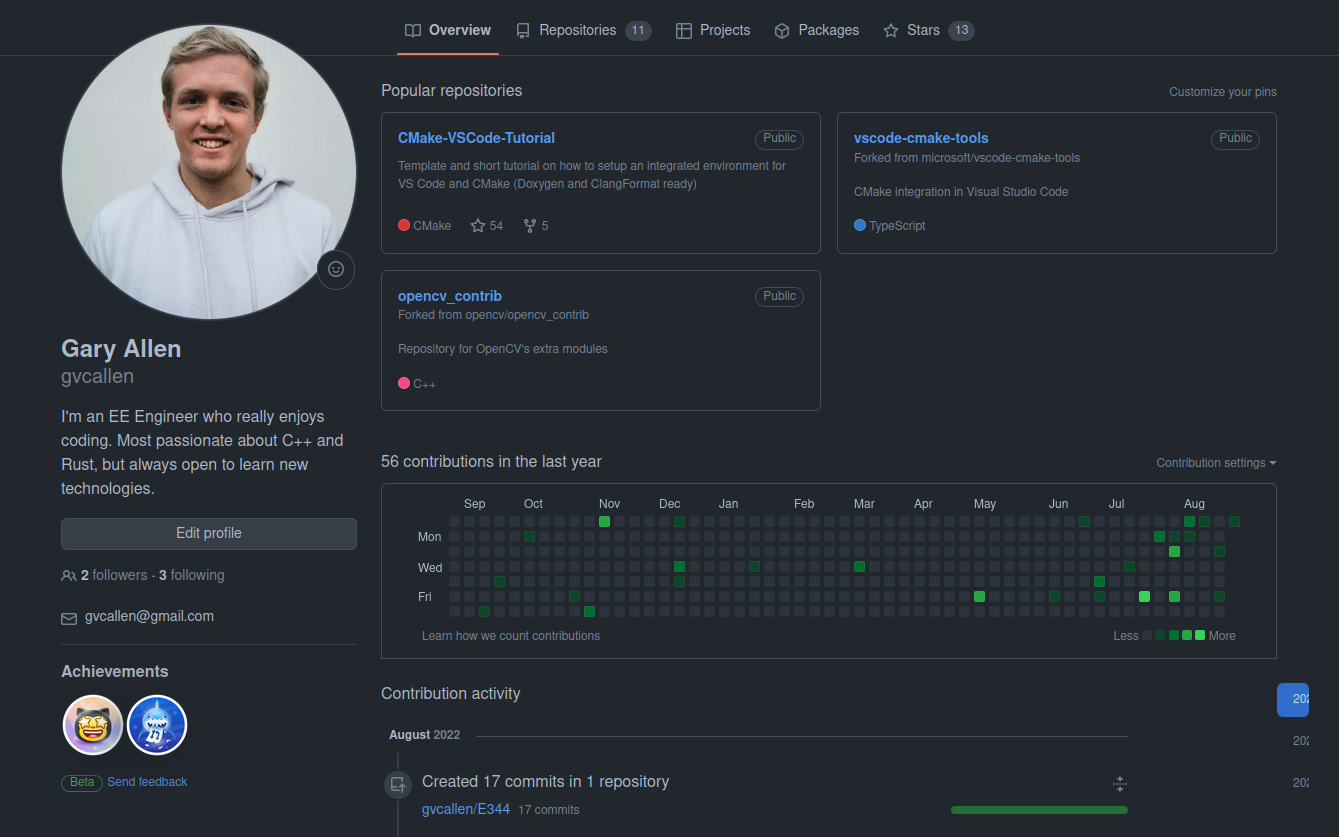
\includegraphics[width=1\linewidth]{GitHub.png}}
	\label{fig:github}
	\end{figure}
\graphicspath{{endmatter/figures/}}
\chapter{Formulae and Derivations}
\makeatletter\@mkboth{}{Appendix}\makeatother

\section{Filters}

\subsection{Common Filter Formulae}{\label{filter_formulae}}
In the following formulae, $f_c$ is the filter's cutoff frequency, $w_c = 2 \pi f_c$, and $H(s)$ is the
Laplace transfer function of the filter. \\

\noindent For a \nth{1} order filter:
\begin{itemize}
\item $H(s) = \frac{w_c}{s + w_c}$
\item Attenuation (dB) $ = -10\log[1 + (\frac{f}{f_{c}})^{2}]$ \cite{pwmAnalogConversion}
\item 10\% to 90\% Rise time, $t_r \approx \frac{2.2}{w_c}$ \cite{firstOrderRiseTime}
\end{itemize}

\noindent For a \nth{2} order filter:
\begin{itemize}
    \item $H(s) = \frac{{w_c}^2}{s^2 + 2 \zeta w_c s + {w_c}^2}$
    \item Attenuation (dB) $ = -10\log [1+(\frac{f}{f_c})^4]$ with $\zeta = 0.707$ [\ref{eqn:2ndOrder_atten_simplified}]
    \item 10\% to 90\% Rise time, $t_r \approx \frac{3.3}{w_c}$ with $\zeta = 0.707$ \cite{gopal2003digital}
\end{itemize}

\noindent For a \nth{3} order filter (formed by cascading a \nth{1} and \nth{2} order):
\begin{itemize}
    \item $H(s) = \left( \frac{w_c}{s + w_c} \right) \left( \frac{{w_c}^2}{s^2 + 2 \zeta w_c s + {w_c}^2} \right)$
    \item Attenuation (dB) $ = -10\log [1+(\frac{f}{f_c})^2+(\frac{f}{f_c})^4+(\frac{f}{f_c})^6] \approx -60\log \left[\frac{f}{f_c}\right]$ with $\zeta = 0.707$ and $f >> f_c$.
    \item 10\% to 90\% Rise time, $t_r \approx \frac{3.97}{w_c}$ with $\zeta = 0.707$, using $t_{ro} = \sqrt{t_{r1}^2 + t_{r2}^2}$ from \cite{cascadedRiseTime}
\end{itemize}

\subsection{\nth{2} Order Filter Attenuation}

For a \nth{2} order filter with the following transfer function:
$$H(s) = \frac{{w_c}^2}{s^2 + 2 \zeta w_c s + {w_c}^2}$$

\noindent The attenuation $A_{dB}$ at frequency $w$ can be calculated as follows:
\begin{align}
    A_{dB} & = 20 \log \left\lvert\frac{w_c^2}{(jw)^2 + 2 \zeta w_c (jw) + w_c^2} \right\rvert                  \notag                                  \\
           & = -20 \log \left\lvert \frac{(w_c^2 - w^2) + j(w 2 \zeta w_c)}{w_c^2} \right\rvert                 \notag                                  \\
           & = -20 \log \sqrt{\frac{w_c ^ 4 - 2 w_c^2 w^2 + w^4 + 4 \zeta ^2 w_c^2 w^2}{w_c^2}}                 \notag                                  \\
           & = -10 \log \left[ \frac{w_c^4 + w^4}{w_c^4} + \frac{w_c^2 w^2 (4 \zeta ^2 - 2)}{w_c^4} \right]     \notag                                  \\
           & = -10 \log \left[ 1 + \left(\frac{w}{w_c}\right)^4 + \left(\frac{w}{w_c}\right)^2 (4 \zeta ^2 - 2) \right] \label{eqn:2ndOrder_atten_full}
\end{align}

For the case when $\zeta = 0.707$ (i.e. when optimally damped), then \ref{eqn:2ndOrder_atten_full} simplifies to:
\begin{equation}
    A = -10 \log \left[1 + \left( \frac{w}{w_c} \right)^4\right] \label{eqn:2ndOrder_atten_simplified}
\end{equation}

\subsection{\nth{1} and \nth{2} Order Filter Cutoff vs Attenuation}

Given:
\begin{itemize}
    \item $f_n = f_{\text{cutoff ($n^{th}$ order)}}$.
    \item For \nth{1} order, attenuation (dB) @ ${f} = -10\log[1 + (\frac{f}{f_{c}})^{2}]$ \cite{pwmAnalogConversion}
    \item For \nth{2} order, attenuation (dB) @ ${f} = -10\log [1+(\frac{f}{f_c})^4]$ with $\zeta = 0.707$ [\ref{eqn:2ndOrder_atten_simplified}]
\end{itemize}


\noindent A \nth{1} order filter will therefore always attenuate a given frequency $f$ less than a \nth{2} order filter with $f_1 = f_2$.
The cutoff frequency of a \nth{2} order filter that will attenuate $f$ by the same amount as a \nth{1} order filter with a given cutoff frequency $f_1$
can be calculated as follows:
\begin{gather}
    -10\log\left[1 + \left(\frac{f}{f_{1}}\right)^{2}\right] = -10\log \left[1+\left(\frac{f}{f_2}\right)^4\right]          \notag\\
    \left( \frac{f}{f_1} \right)^2 = \left( \frac{f}{f_2} \right)^4                                                         \notag\\
    \therefore f_2^4 = \frac{f^4}{f^2} f_1^2                                                                                \notag\\
    \therefore f_2^4 = f^2 f_1^2                                                                                            \notag\\
    \therefore f_2 = \sqrt{f \cdot f_1}                                                                                     \label{eqn:1st2nd_cutoff_atten}
\end{gather}

\end{document}